
\section{Експериментални резултати}

\subsection{Цел на упражнението}

Целта на това упражнение е да се изследват основни методи за анализ и подобряване на цифрови изображения. Изследват се хистограмите като инструмент за оценка на яркостта и контраста, линейни и нелинейни контрастни трансформации (imadjust и $\gamma$-корекция), пространствени изглаждащи филтри (осредняващ, Гаусов и медианен) и метода за засилване на рязкостта чрез Unsharp Masking. Всеки метод се прилага върху реални изображения и резултатите се анализират качествено.

\section{Резултати и анализ по задания}

\subsection{Задание 1 – Хистограма на изображение}

\subsubsection{Код}

\begin{lstlisting}[language=Matlab, caption={task1\_histogram.m}]
pkg load image;
clear; close all;

img_dir = '../images/';
out_dir = '../results/';
images = {'Img17', 'Img18', 'Img19', 'Img21', 'Img24'};

num_bins = 256;
bin_range = [0, 255];

stats = zeros(length(images), 2);

for k = 1:length(images)
    name = images{k};
    img = imread([img_dir name '.tif']);

    if size(img, 3) == 3
        img_gray = rgb2gray(img);
    else
        img_gray = img;
    end

    img_gray = im2uint8(img_gray);

    stats(k, 1) = mean(double(img_gray(:)));
    stats(k, 2) = std(double(img_gray(:)));

    fig = figure('visible', 'off', 'Position', [0 0 900 400]);
    subplot(1, 2, 1);
    imshow(img_gray);
    title([name ' - original']);

    subplot(1, 2, 2);
    centers = 0:255;
    counts = histc(double(img_gray(:)), centers);
    bar(centers, counts, 1, 'FaceColor', [0.3 0.3 0.8], 'EdgeColor', 'none');
    xlim(bin_range);
    xlabel('Intensity');
    ylabel('Pixel count');
    title([name ' - histogram']);

    saveas(fig, [out_dir 'task1_subplot_' name '.png']);
    close(fig);
end
\end{lstlisting}

\subsubsection{Резултати}

За всяко от петте изображения е построена фигура тип subplot – вляво оригиналното изображение, вдясно съответната хистограма. Използвани са еднакви настройки: 256 бина и диапазон $[0, 255]$.

\begin{figure}[H]
    \centering
    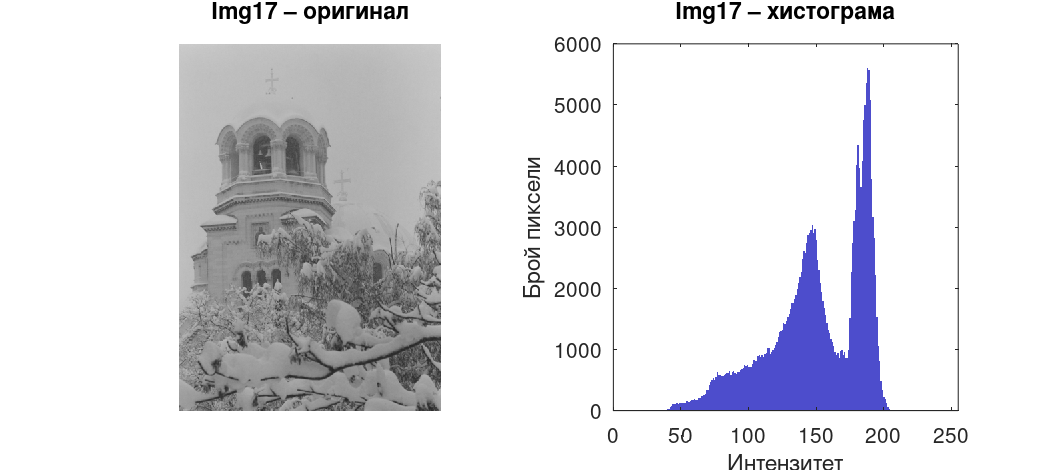
\includegraphics[width=0.95\textwidth]{../results/task1_subplot_Img17.png}
    \caption{Img17 – оригинал и хистограма}
\end{figure}

\begin{figure}[H]
    \centering
    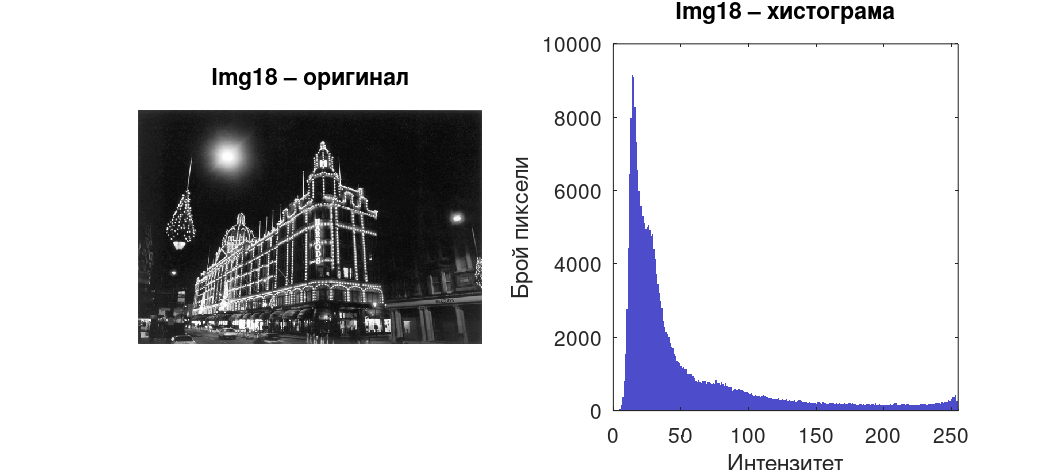
\includegraphics[width=0.95\textwidth]{../results/task1_subplot_Img18.png}
    \caption{Img18 – оригинал и хистограма}
\end{figure}

\begin{figure}[H]
    \centering
    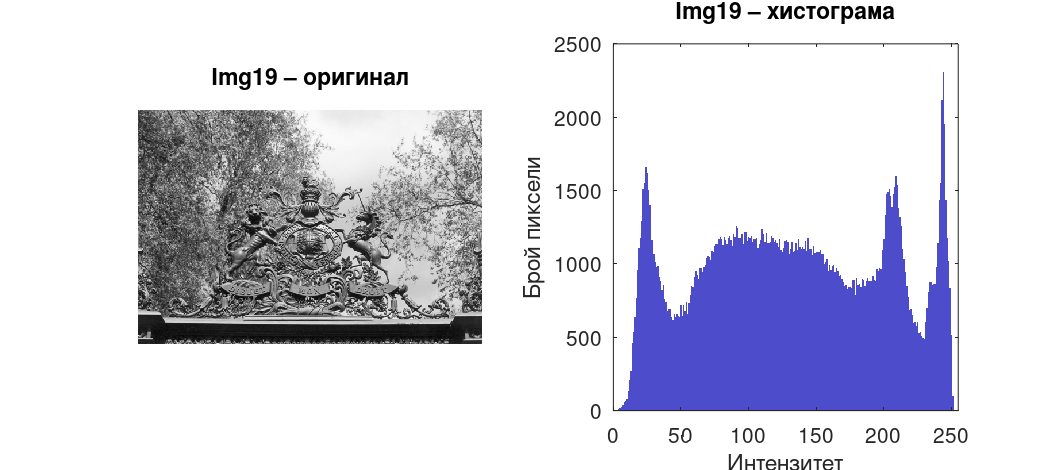
\includegraphics[width=0.95\textwidth]{../results/task1_subplot_Img19.png}
    \caption{Img19 – оригинал и хистограма}
\end{figure}

\begin{figure}[H]
    \centering
    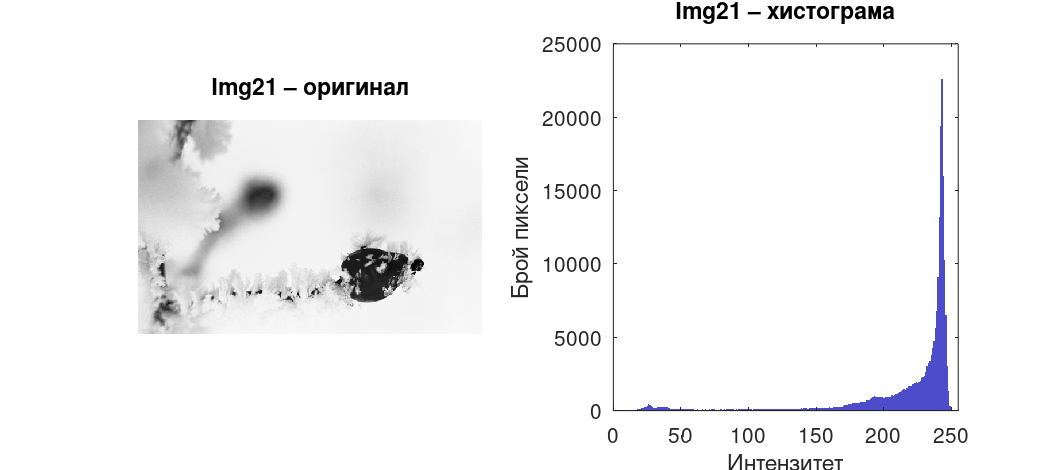
\includegraphics[width=0.95\textwidth]{../results/task1_subplot_Img21.png}
    \caption{Img21 – оригинал и хистограма}
\end{figure}

\begin{figure}[H]
    \centering
    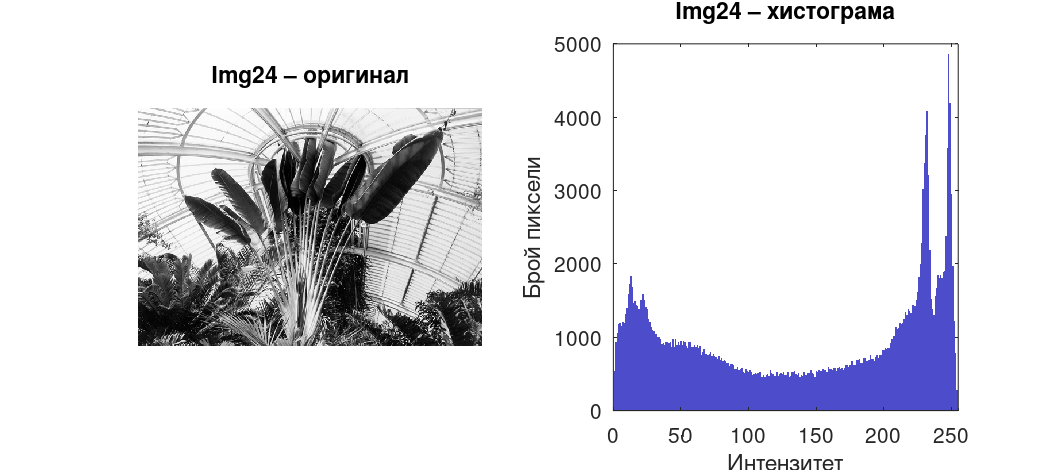
\includegraphics[width=0.95\textwidth]{../results/task1_subplot_Img24.png}
    \caption{Img24 – оригинал и хистограма}
\end{figure}

\noindent Таблица с оценка на яркостта и контраста по изображения (изчислени като средна стойност и стандартно отклонение на пикселните интензитети):

\begin{table}[H]
\centering
\caption{Оценка на яркост и контраст}
\begin{tabular}{lllll}
\toprule
\textbf{Изображение} & \textbf{Яркост (mean)} & \textbf{Контраст (std)} & \textbf{Клас яркост} & \textbf{Клас контраст} \\
\midrule
Img17 & 150.89 & 35.26 & Средна & Нисък \\
Img18 & 52.42  & 54.94 & Тъмна  & Среден \\
Img19 & 132.45 & 67.83 & Средна & Среден \\
Img21 & 218.55 & 45.54 & Светла & Среден \\
Img24 & 141.43 & 86.60 & Средна & Висок \\
\bottomrule
\end{tabular}
\end{table}

\subsubsection{Анализ}

\textbf{Класификация по яркост и контраст:} Img18 е най-тъмното изображение (mean~=~52), а Img21 е най-светлото (mean~=~218). Img24 има най-висок контраст (std~=~86), докато Img17 показва нисък контраст (std~=~35).

\textbf{Положение на хистограмата и яркост:} Хистограма, струпана в лявата (тъмна) страна, съответства на тъмно изображение; струпана вдясно – на светло изображение. Img18 има хистограма концентрирана в ниските интензитети, а Img21 – в горните.

\textbf{Ширина на хистограмата и контраст:} Широка хистограма (покриваща целия диапазон) означава висок контраст – много тъмни и много светли области едновременно. Img24 демонстрира това поведение. Тясна хистограма (Img17) означава малка разлика между най-тъмния и най-светлия пиксел.

\textbf{Сравнение на сходни хистограми:} Img17 и Img21 имат сходно стандартно отклонение (около 35–45), но различна средна яркост. Img17 е средно яркото, Img21 е светло. Разликата се дължи на различното разпределение на светлите тонове – Img21 съдържа предимно бели/светли повърхности, докато Img17 има балансирани средни тонове. Локалното разпределение и структурата на обектите в изображението са определящи.

\subsection{Задание 2 – Разширяване на динамичния обхват (imadjust и $\gamma$-корекция)}

\subsubsection{Код}

\begin{lstlisting}[language=Matlab, caption={task2\_contrast.m}]
pkg load image;
clear; close all;

img_dir = '../images/';
out_dir = '../results/';
images = {'Img21', 'Img24'};
gammas = [0.6, 1.0, 1.6];

for k = 1:length(images)
    name = images{k};
    img = imread([img_dir name '.tif']);

    if size(img, 3) == 3
        img_gray = rgb2gray(img);
    else
        img_gray = img;
    end
    img_gray = im2uint8(img_gray);

    img_adj = imadjust(img_gray);

    img_gamma = cell(1, length(gammas));
    for g = 1:length(gammas)
        gamma = gammas(g);
        img_norm = double(img_gray) / 255;
        img_corrected = img_norm .^ gamma;
        img_gamma{g} = im2uint8(img_corrected);
    end

    imwrite(img_gray,     [out_dir 'task2_original_'  name '.png']);
    imwrite(img_adj,      [out_dir 'task2_imadjust_'  name '.png']);
    imwrite(img_gamma{1}, [out_dir 'task2_gamma06_'   name '.png']);
    imwrite(img_gamma{2}, [out_dir 'task2_gamma10_'   name '.png']);
    imwrite(img_gamma{3}, [out_dir 'task2_gamma16_'   name '.png']);

    fig = figure('visible', 'off', 'Position', [0 0 1400 400]);
    titles = {[name ' original'], 'imadjust', 'gamma=0.6', 'gamma=1.0', 'gamma=1.6'};
    imgs   = {img_gray, img_adj, img_gamma{1}, img_gamma{2}, img_gamma{3}};
    for i = 1:5
        subplot(1, 5, i);
        imshow(imgs{i});
        title(titles{i});
    end
    saveas(fig, [out_dir 'task2_comparison_' name '.png']);
    close(fig);
end
\end{lstlisting}

\subsubsection{Резултати}

За изображенията Img21 и Img24 са приложени: imadjust (линейно разтягане на хистограмата) и $\gamma$-корекция при $\gamma = 0.6$, $\gamma = 1.0$ и $\gamma = 1.6$.

\begin{figure}[H]
    \centering
    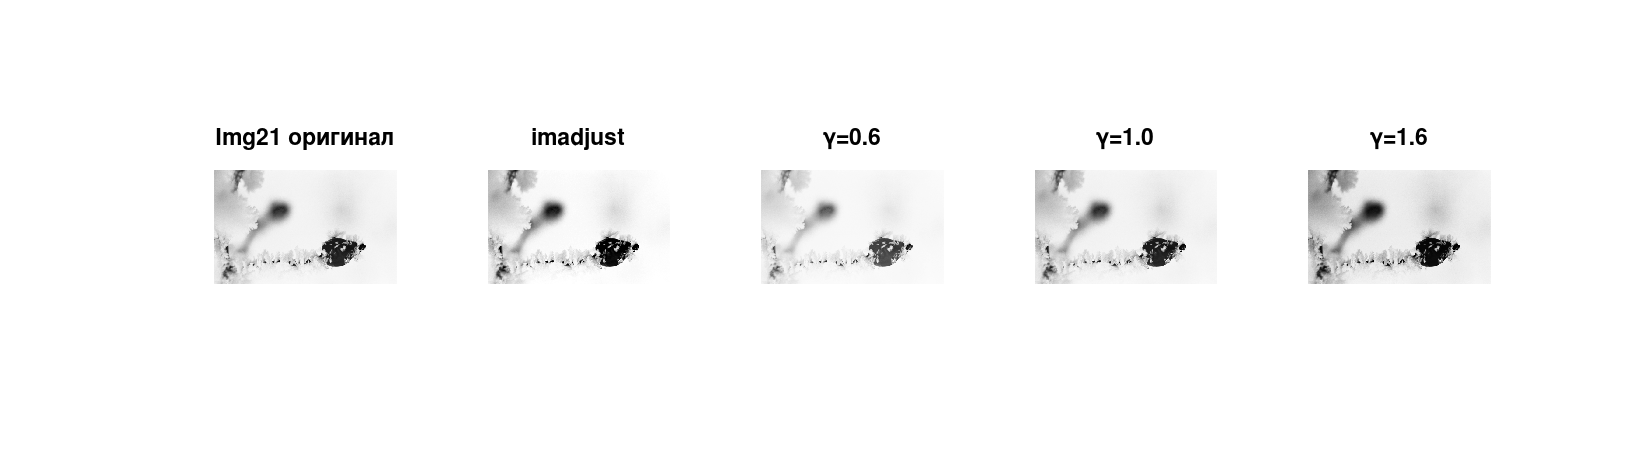
\includegraphics[width=\textwidth]{../results/task2_comparison_Img21.png}
    \caption{Img21 – сравнение: оригинал, imadjust, $\gamma=0.6$, $\gamma=1.0$, $\gamma=1.6$}
\end{figure}

\begin{figure}[H]
    \centering
    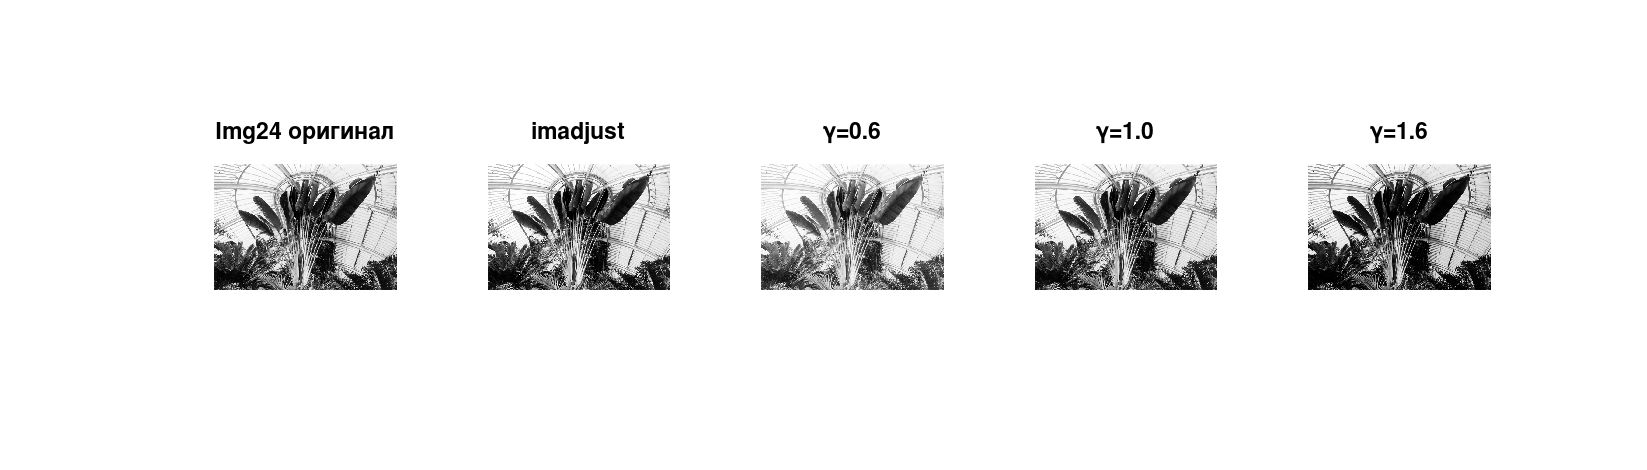
\includegraphics[width=\textwidth]{../results/task2_comparison_Img24.png}
    \caption{Img24 – сравнение: оригинал, imadjust, $\gamma=0.6$, $\gamma=1.0$, $\gamma=1.6$}
\end{figure}

\noindent Хистограми преди и след обработка:

\begin{figure}[H]
    \centering
    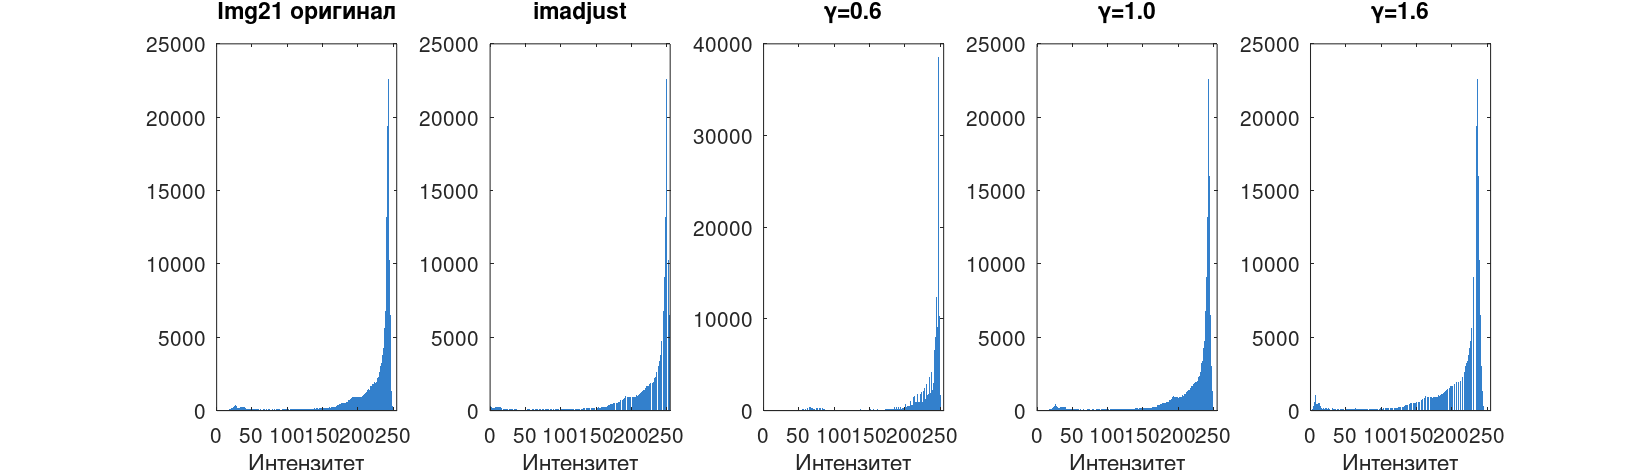
\includegraphics[width=\textwidth]{../results/task2_histograms_Img21.png}
    \caption{Img21 – хистограми: оригинал, imadjust, $\gamma=0.6$, $\gamma=1.0$, $\gamma=1.6$}
\end{figure}

\begin{figure}[H]
    \centering
    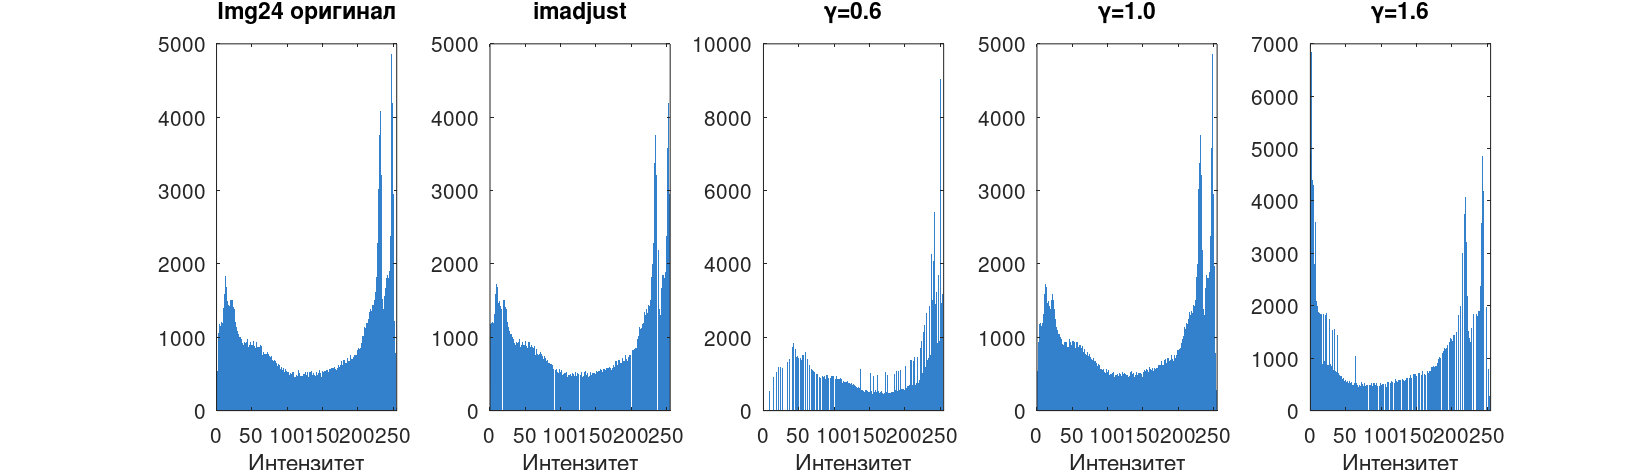
\includegraphics[width=\textwidth]{../results/task2_histograms_Img24.png}
    \caption{Img24 – хистограми: оригинал, imadjust, $\gamma=0.6$, $\gamma=1.0$, $\gamma=1.6$}
\end{figure}

\subsubsection{Анализ}

\textbf{Промяна на хистограмата след imadjust:} imadjust извършва линейно разтягане на интензитетите към целия диапазон $[0, 255]$. Хистограмата се разпростира по-широко и контрастът се увеличава. При Img21 (светло изображение) разтягането е по-видимо в тъмните области.

\textbf{Ефект на $\gamma < 1$ ($\gamma = 0.6$):} Нелинейно усилване на тъмните области – тъмните пиксели стават по-светли. Светлите области се засягат по-малко. Хистограмата се измества наляво (тъмни пиксели) и се „разтяга" в светлата зона.

\textbf{Ефект на $\gamma > 1$ ($\gamma = 1.6$):} Потъмняване на изображението – тъмните области стават още по-тъмни, светлите се засягат по-малко. Детайлите в сенките се губят. Хистограмата се измества надясно (по-ниски стойности).

\textbf{Най-подходяща стойност на $\gamma$:} За Img21 (светло изображение, детайли в сенките) най-подходяща е $\gamma = 0.6$ – засилва тъмните зони и позволява разграничаване на детайли в сенките. За Img24 (средна яркост, висок контраст) $\gamma = 0.6$ също е подходяща за изявяване на тъмните текстури.

\textbf{Пример за неподходяща $\gamma$-корекция:} $\gamma = 1.6$ при Img21 (вече светло изображение) води до прекомерно потъмняване и загуба на детайли в тъмните области. $\gamma = 0.6$ при Img21 може да доведе до преосветяване на вече светлите зони.

\subsection{Задание 3 – Сравнение на изглаждащи пространствени филтри}

\subsubsection{Код}

\begin{lstlisting}[language=Matlab, caption={task3\_filters.m}]
pkg load image;
clear; close all;

img_dir = '../images/';
out_dir = '../results/';
images = {'America', 'SantaMaria'};

for k = 1:length(images)
    name = images{k};
    img = imread([img_dir name '.tif']);

    function result = apply_filter_img(img, filt_func)
        if size(img, 3) == 3
            result = cat(3, filt_func(img(:,:,1)), ...
                            filt_func(img(:,:,2)), ...
                            filt_func(img(:,:,3)));
        else
            result = filt_func(img);
        end
    end

    h5   = fspecial('average', [5 5]);
    h11  = fspecial('average', [11 11]);
    img_mean5  = apply_filter_img(img, @(x) imfilter(x, h5,  'replicate'));
    img_mean11 = apply_filter_img(img, @(x) imfilter(x, h11, 'replicate'));

    hg08 = fspecial('gaussian', [15 15], 0.8);
    hg18 = fspecial('gaussian', [21 21], 1.8);
    img_gauss08 = apply_filter_img(img, @(x) imfilter(x, hg08, 'replicate'));
    img_gauss18 = apply_filter_img(img, @(x) imfilter(x, hg18, 'replicate'));

    img_med3 = apply_filter_img(img, @(x) medfilt2(x, [3 3]));
    img_med7 = apply_filter_img(img, @(x) medfilt2(x, [7 7]));

    imwrite(img,         [out_dir 'task3_original_'  name '.png']);
    imwrite(img_mean5,   [out_dir 'task3_mean5_'     name '.png']);
    imwrite(img_mean11,  [out_dir 'task3_mean11_'    name '.png']);
    imwrite(img_gauss08, [out_dir 'task3_gauss08_'   name '.png']);
    imwrite(img_gauss18, [out_dir 'task3_gauss18_'   name '.png']);
    imwrite(img_med3,    [out_dir 'task3_median3_'   name '.png']);
    imwrite(img_med7,    [out_dir 'task3_median7_'   name '.png']);

    fig = figure('visible', 'off', 'Position', [0 0 1800 700]);
    all_imgs   = {img, img_mean5, img_mean11, img_gauss08, img_gauss18, img_med3, img_med7};
    all_titles = {'Original', 'Mean 5x5', 'Mean 11x11', ...
                  'Gauss s=0.8', 'Gauss s=1.8', 'Median 3x3', 'Median 7x7'};
    for i = 1:7
        subplot(2, 4, i);
        imshow(all_imgs{i});
        title(all_titles{i});
    end
    saveas(fig, [out_dir 'task3_comparison_' name '.png']);
    close(fig);
end
\end{lstlisting}

\subsubsection{Резултати}

За America.tif и SantaMaria.tif са приложени осредняващ филтър (5$\times$5 и 11$\times$11), Гаусов филтър ($\sigma=0.8$ и $\sigma=1.8$) и медианен филтър (3$\times$3 и 7$\times$7). Цветните изображения са обработени по канали (R, G, B).

\begin{figure}[H]
    \centering
    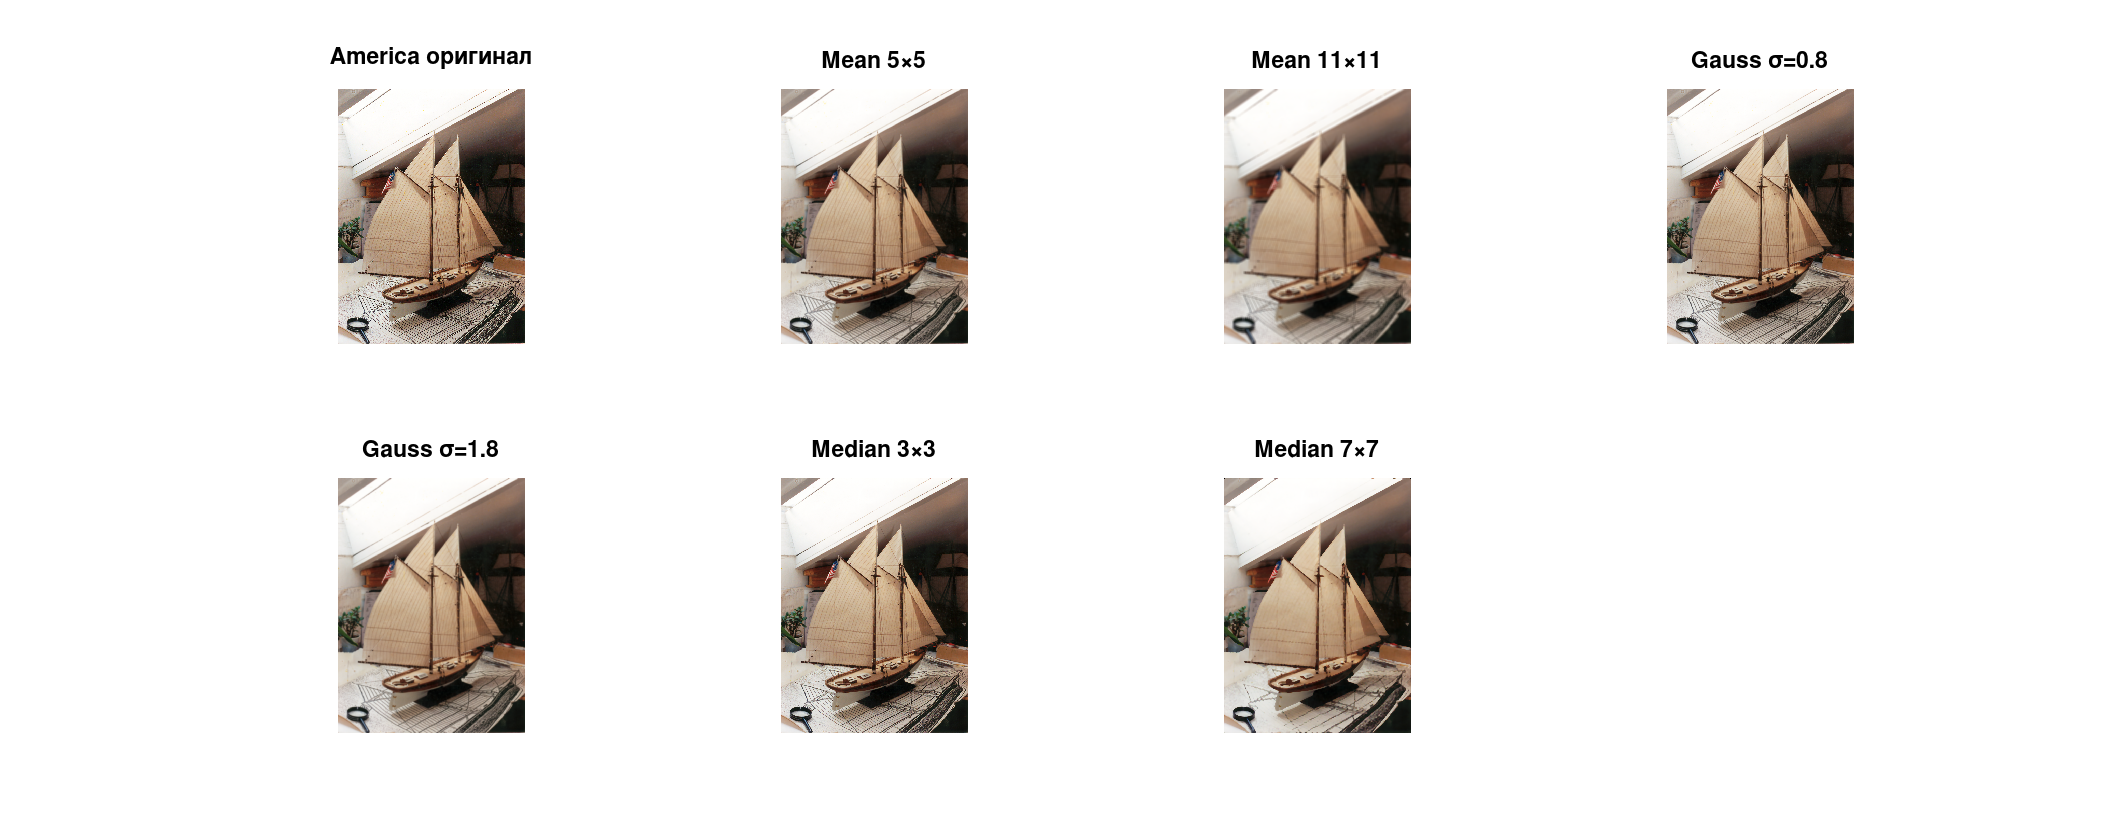
\includegraphics[width=\textwidth]{../results/task3_comparison_America.png}
    \caption{America.tif – сравнение на всички филтри}
\end{figure}

\begin{figure}[H]
    \centering
    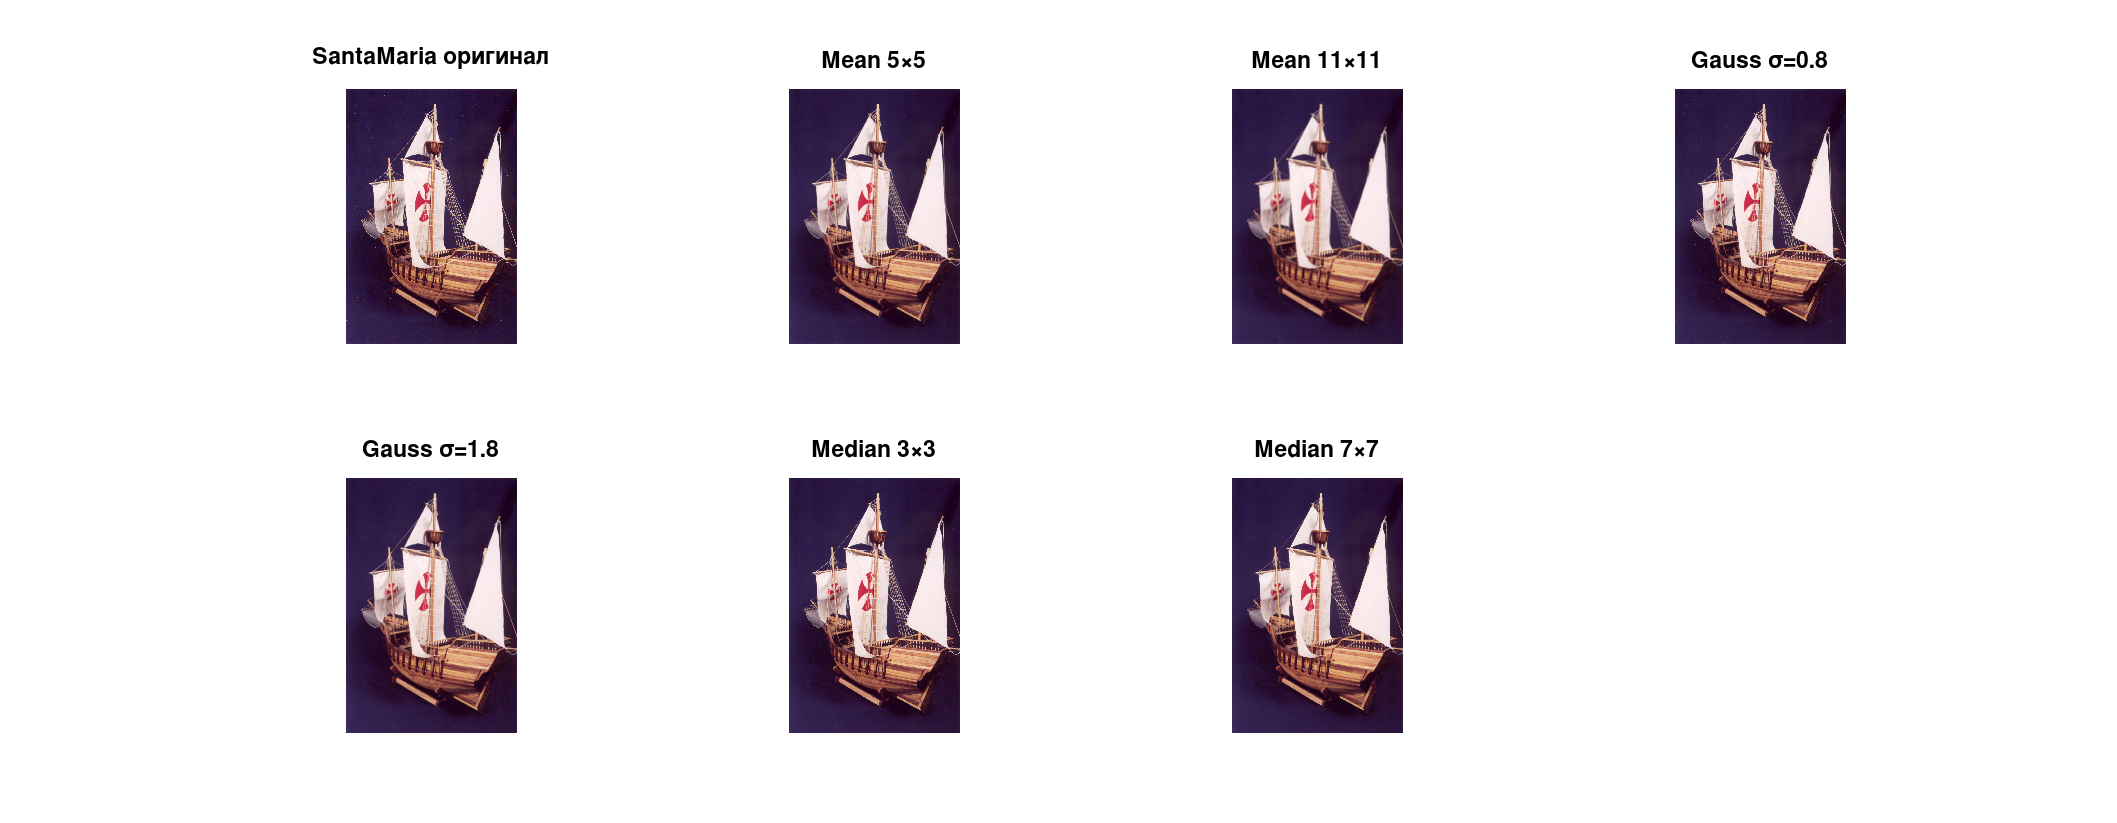
\includegraphics[width=\textwidth]{../results/task3_comparison_SantaMaria.png}
    \caption{SantaMaria.tif – сравнение на всички филтри}
\end{figure}

\noindent Индивидуални резултати за America.tif:

\begin{figure}[H]
    \centering
    \begin{subfigure}[b]{0.32\textwidth}
        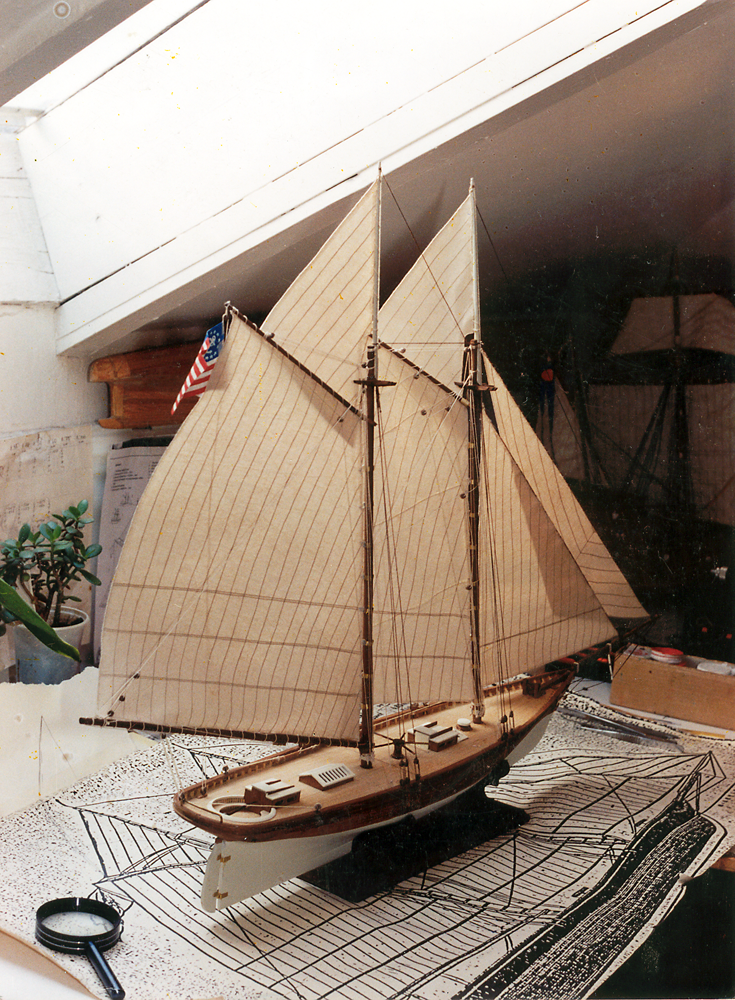
\includegraphics[width=\textwidth]{../results/task3_original_America.png}
        \caption{Оригинал}
    \end{subfigure}
    \begin{subfigure}[b]{0.32\textwidth}
        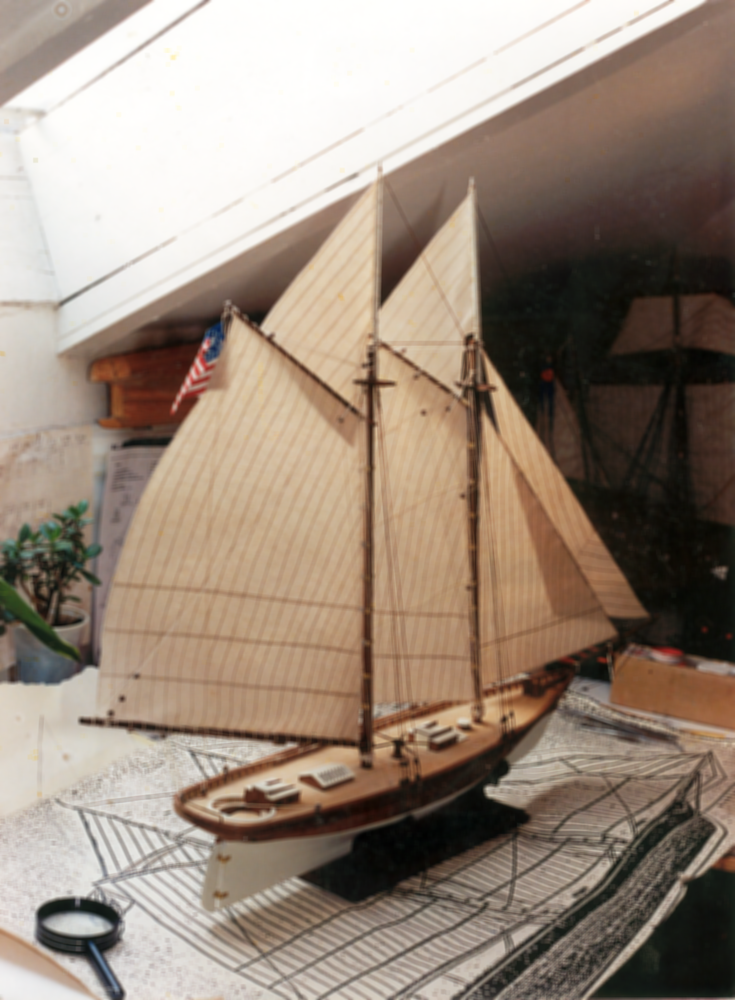
\includegraphics[width=\textwidth]{../results/task3_mean5_America.png}
        \caption{Mean 5$\times$5}
    \end{subfigure}
    \begin{subfigure}[b]{0.32\textwidth}
        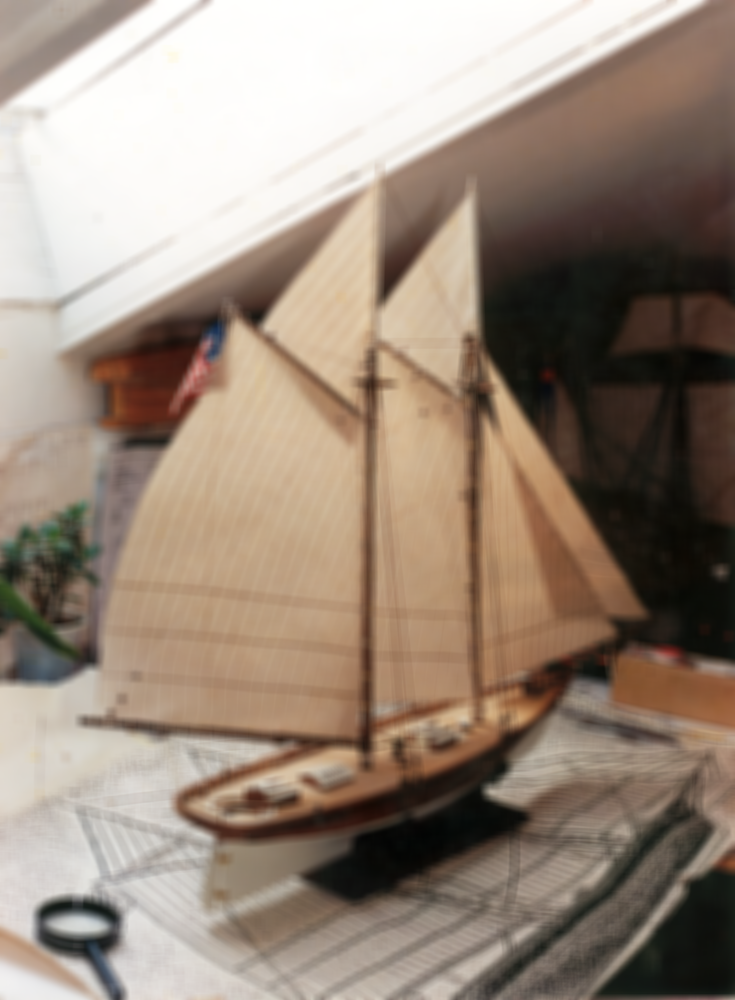
\includegraphics[width=\textwidth]{../results/task3_mean11_America.png}
        \caption{Mean 11$\times$11}
    \end{subfigure}
    \begin{subfigure}[b]{0.32\textwidth}
        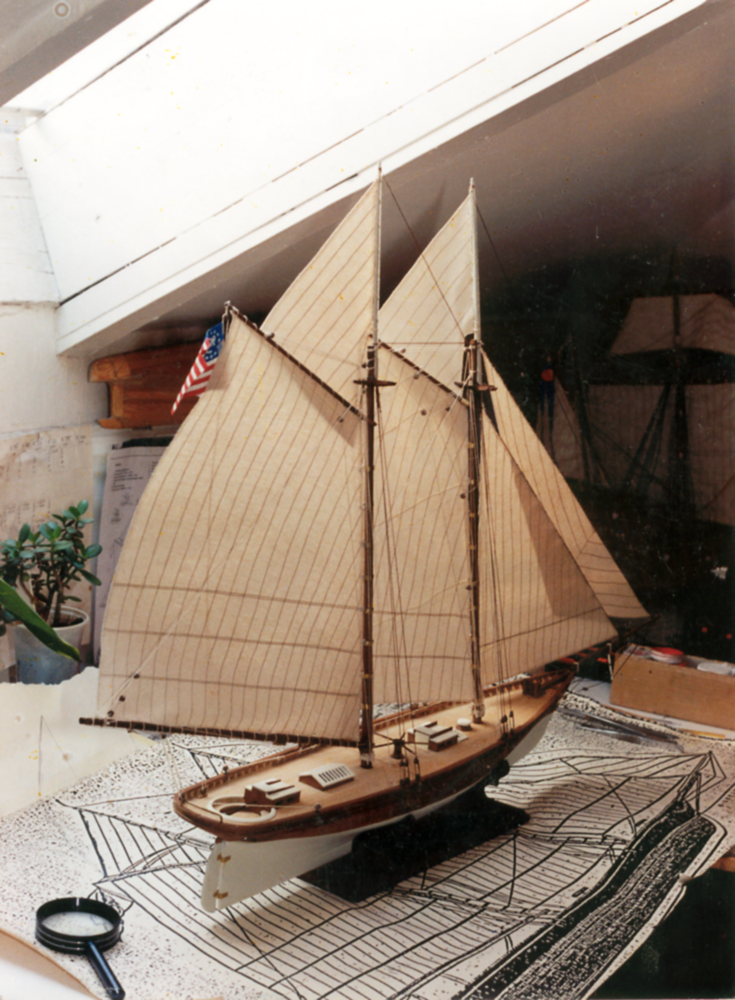
\includegraphics[width=\textwidth]{../results/task3_gauss08_America.png}
        \caption{Gauss $\sigma=0.8$}
    \end{subfigure}
    \begin{subfigure}[b]{0.32\textwidth}
        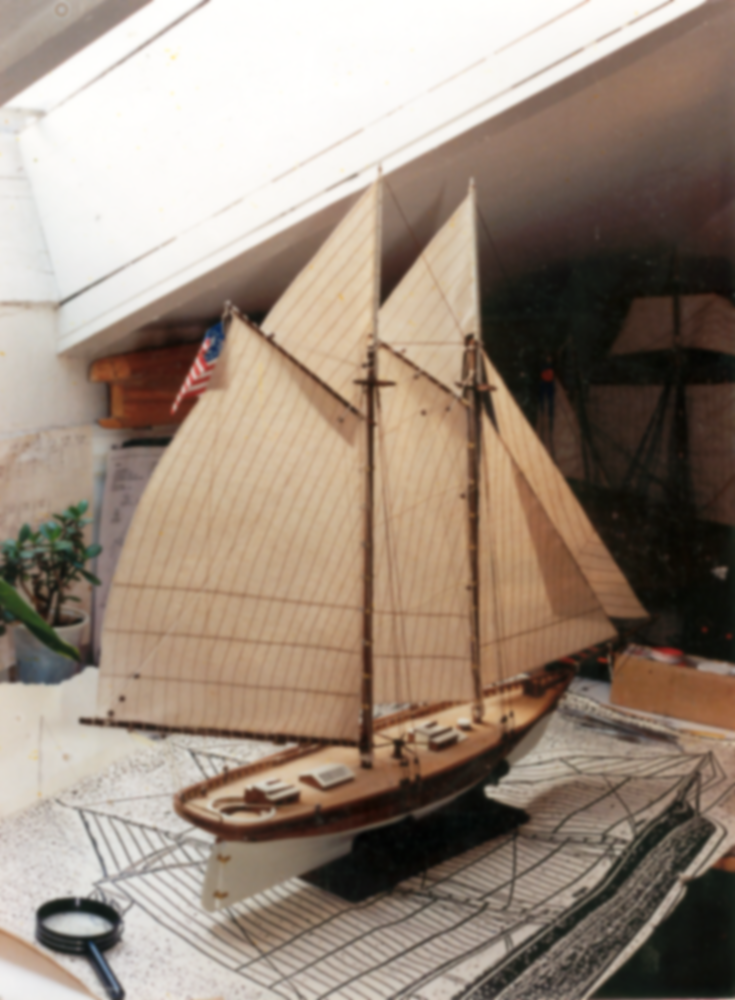
\includegraphics[width=\textwidth]{../results/task3_gauss18_America.png}
        \caption{Gauss $\sigma=1.8$}
    \end{subfigure}
    \begin{subfigure}[b]{0.32\textwidth}
        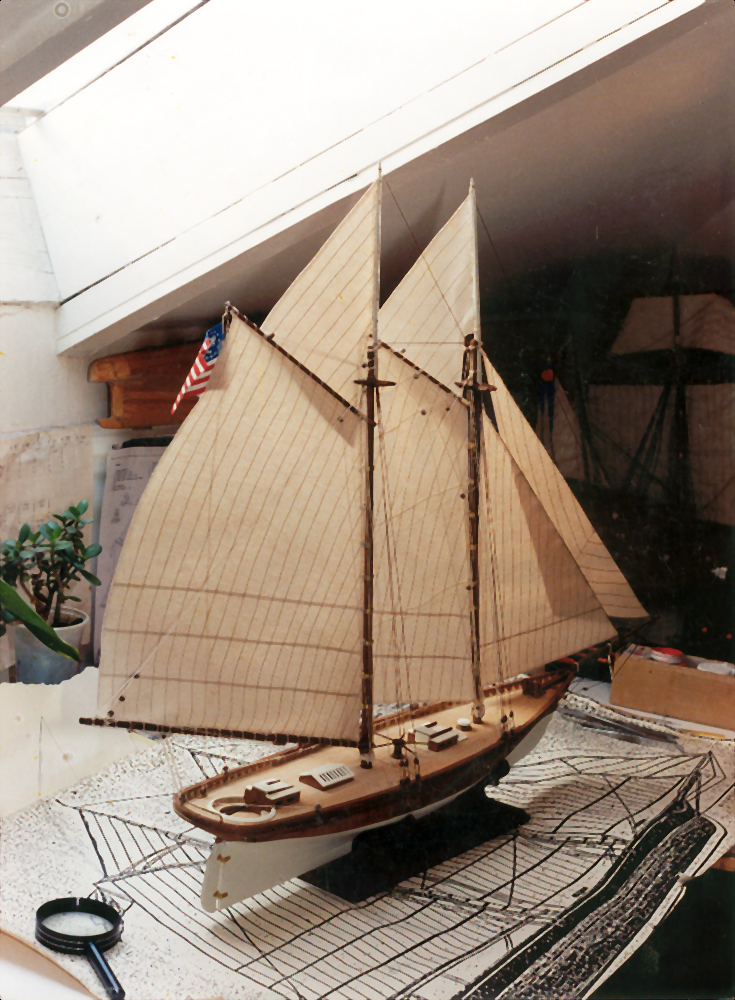
\includegraphics[width=\textwidth]{../results/task3_median3_America.png}
        \caption{Median 3$\times$3}
    \end{subfigure}
    \caption{America.tif – индивидуални резултати от филтриране}
\end{figure}

\begin{figure}[H]
    \centering
    \begin{subfigure}[b]{0.32\textwidth}
        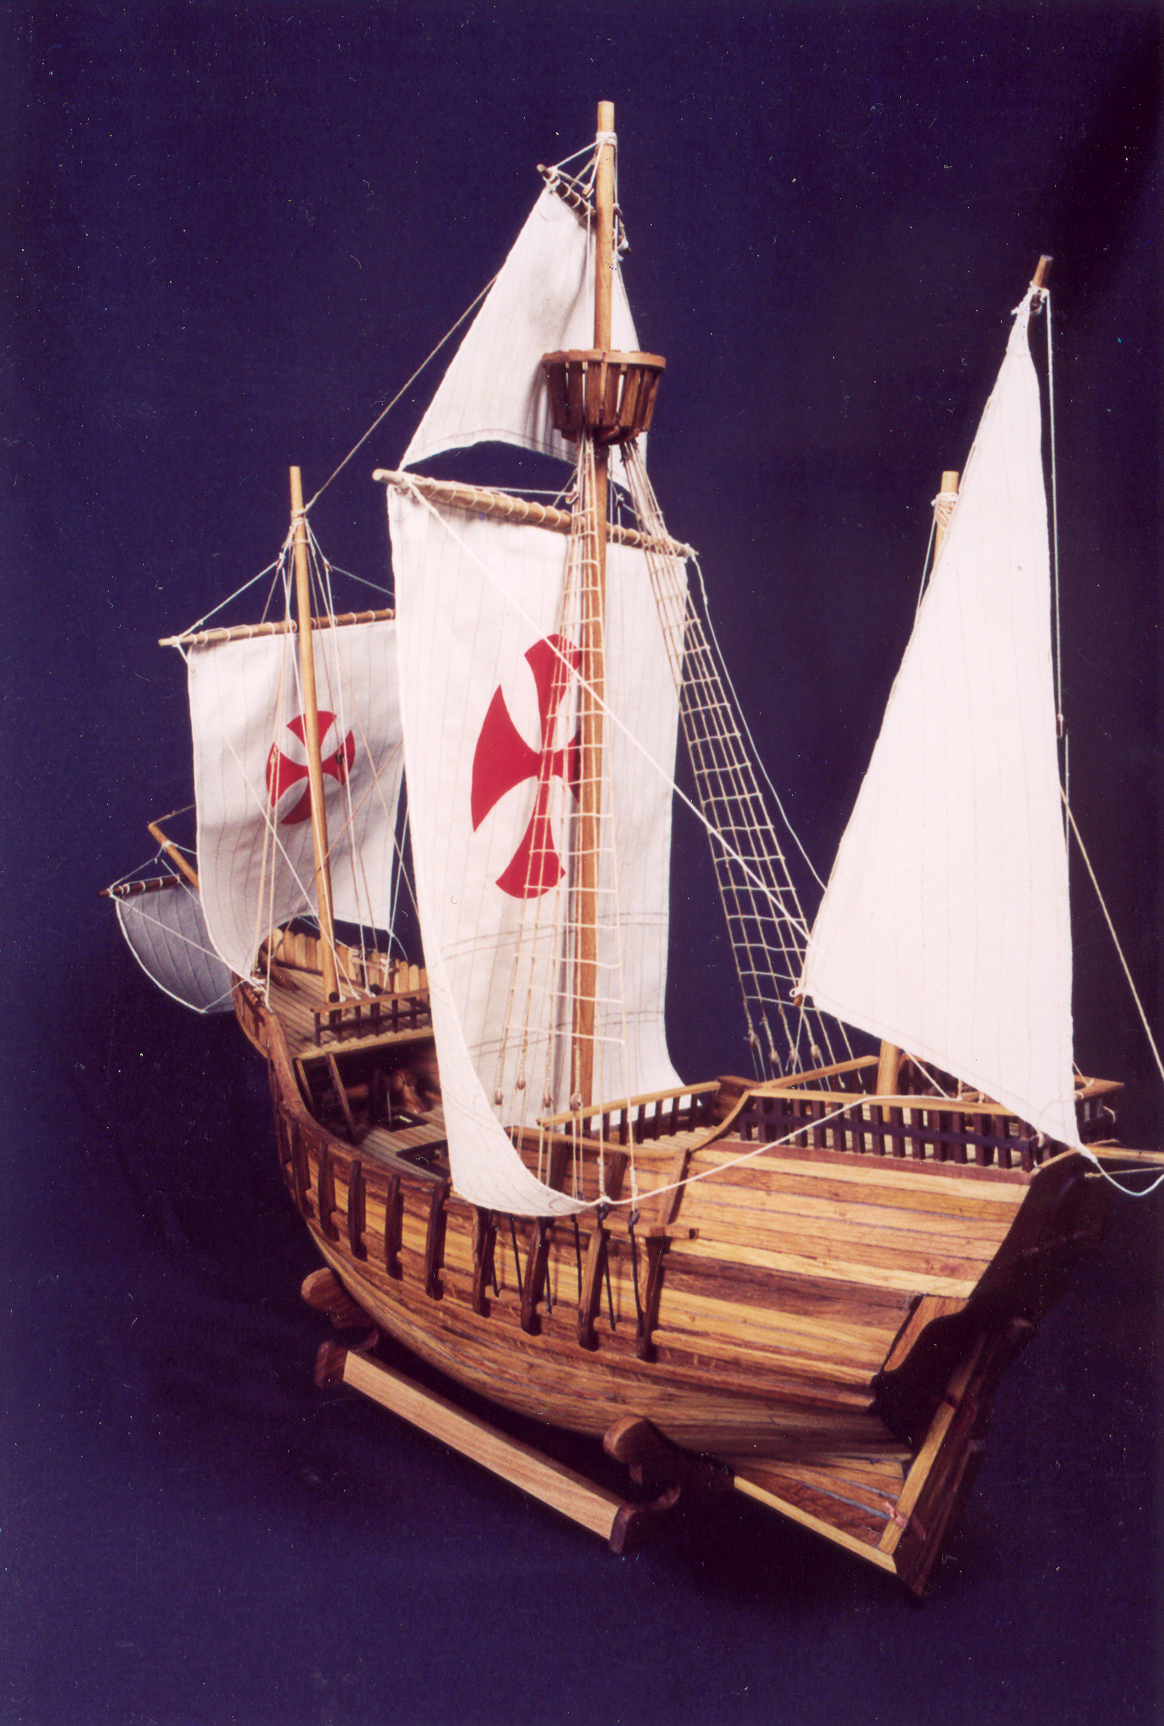
\includegraphics[width=\textwidth]{../results/task3_original_SantaMaria.png}
        \caption{Оригинал}
    \end{subfigure}
    \begin{subfigure}[b]{0.32\textwidth}
        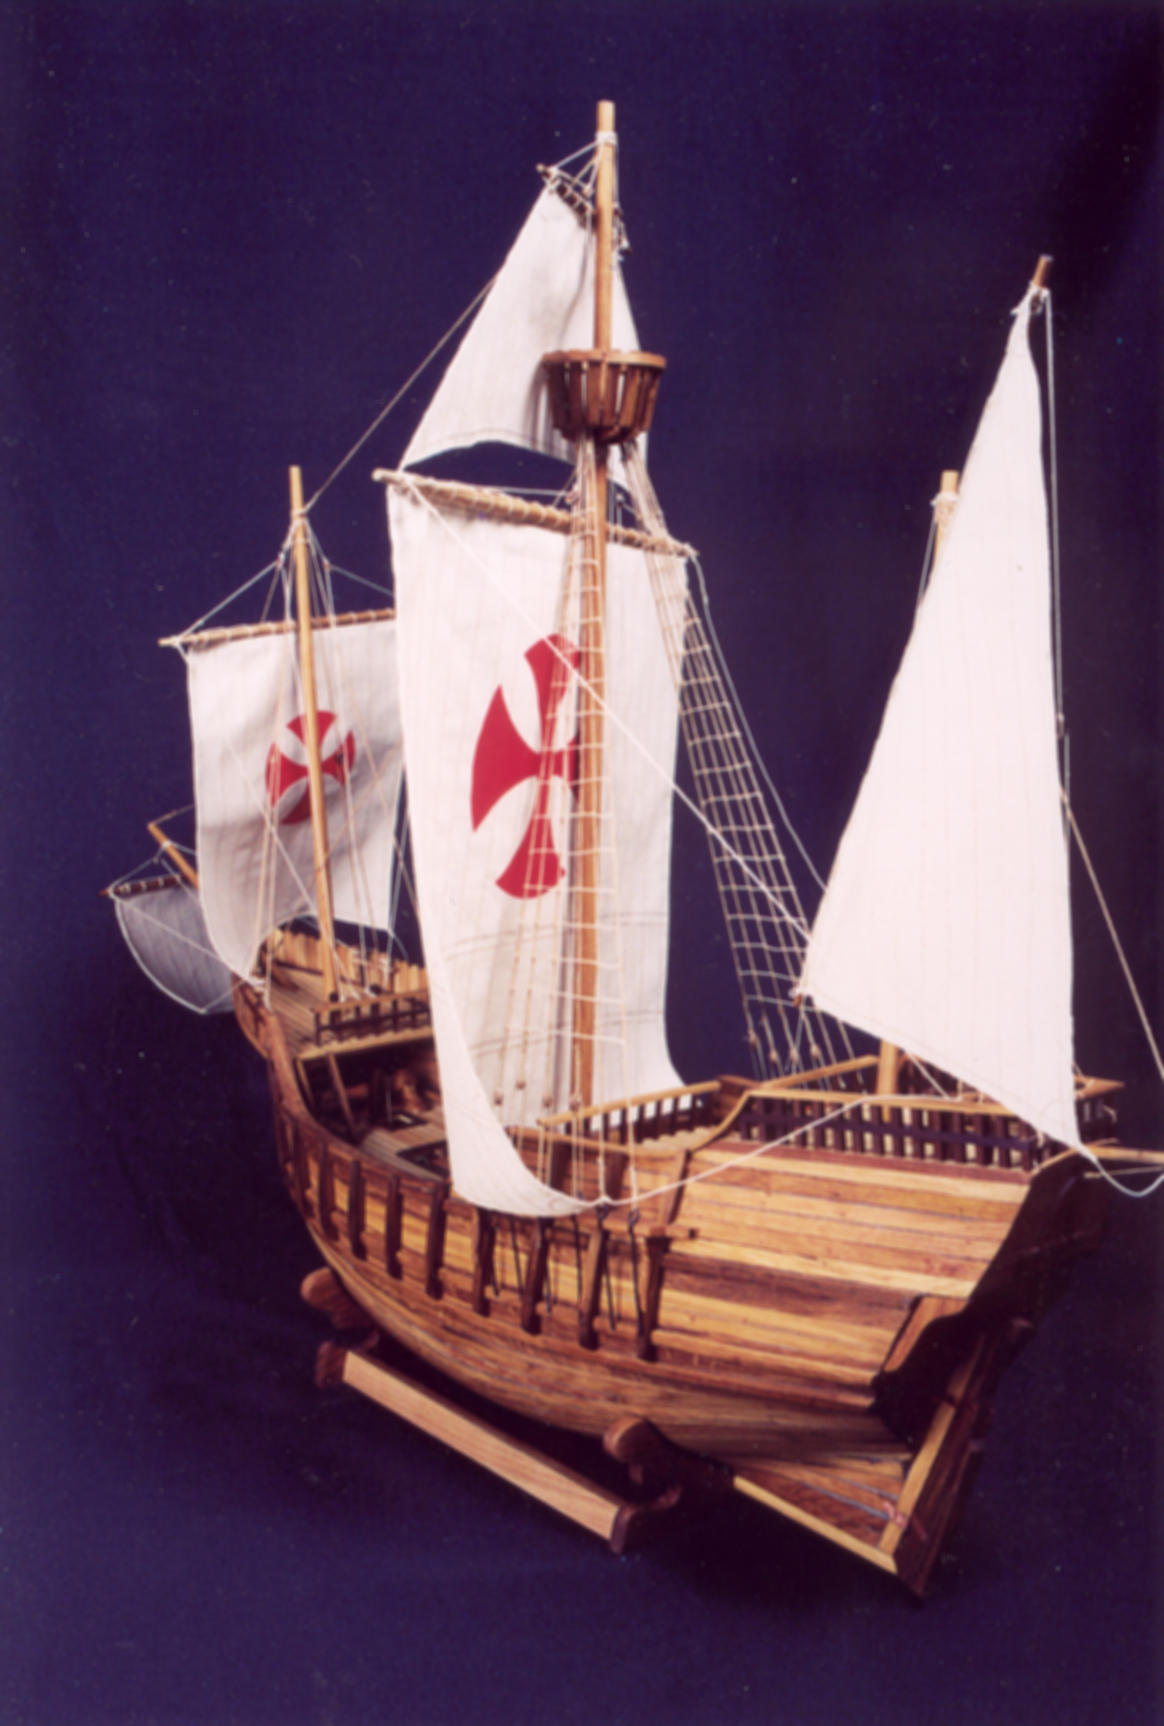
\includegraphics[width=\textwidth]{../results/task3_mean5_SantaMaria.png}
        \caption{Mean 5$\times$5}
    \end{subfigure}
    \begin{subfigure}[b]{0.32\textwidth}
        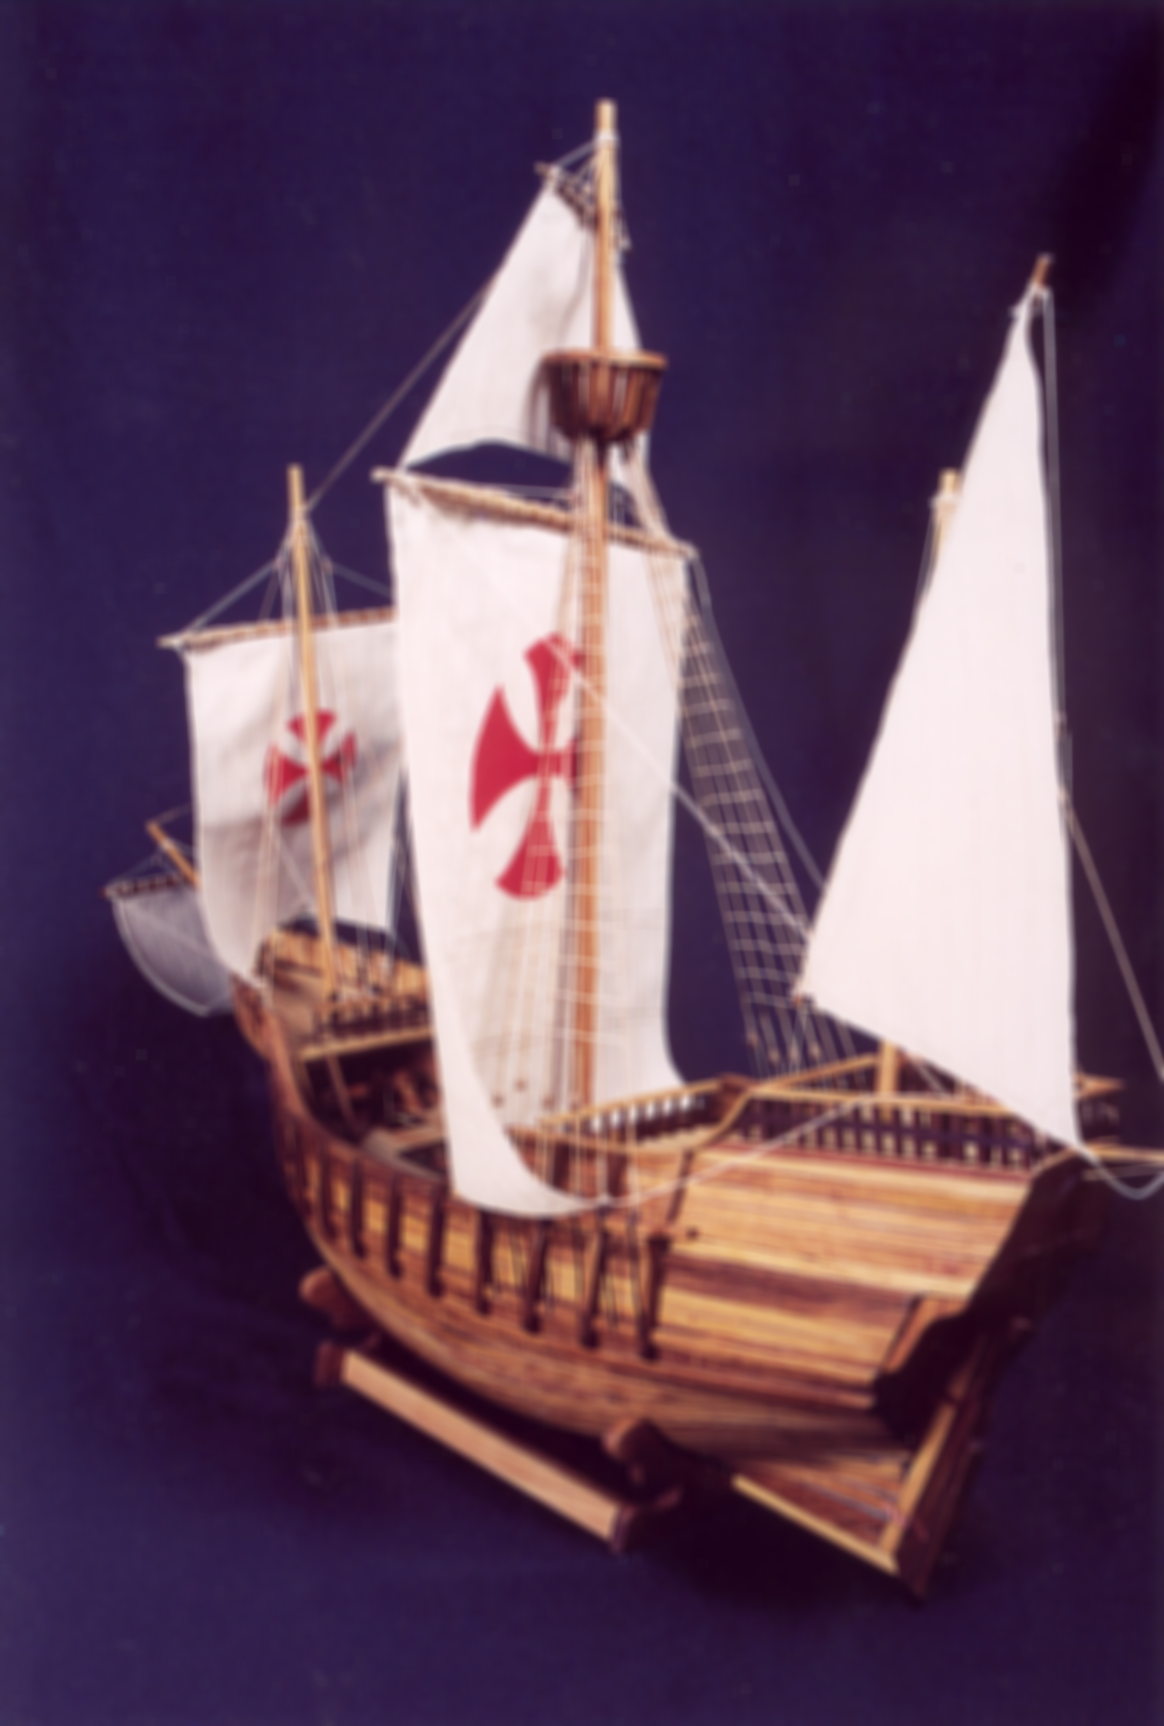
\includegraphics[width=\textwidth]{../results/task3_mean11_SantaMaria.png}
        \caption{Mean 11$\times$11}
    \end{subfigure}
    \begin{subfigure}[b]{0.32\textwidth}
        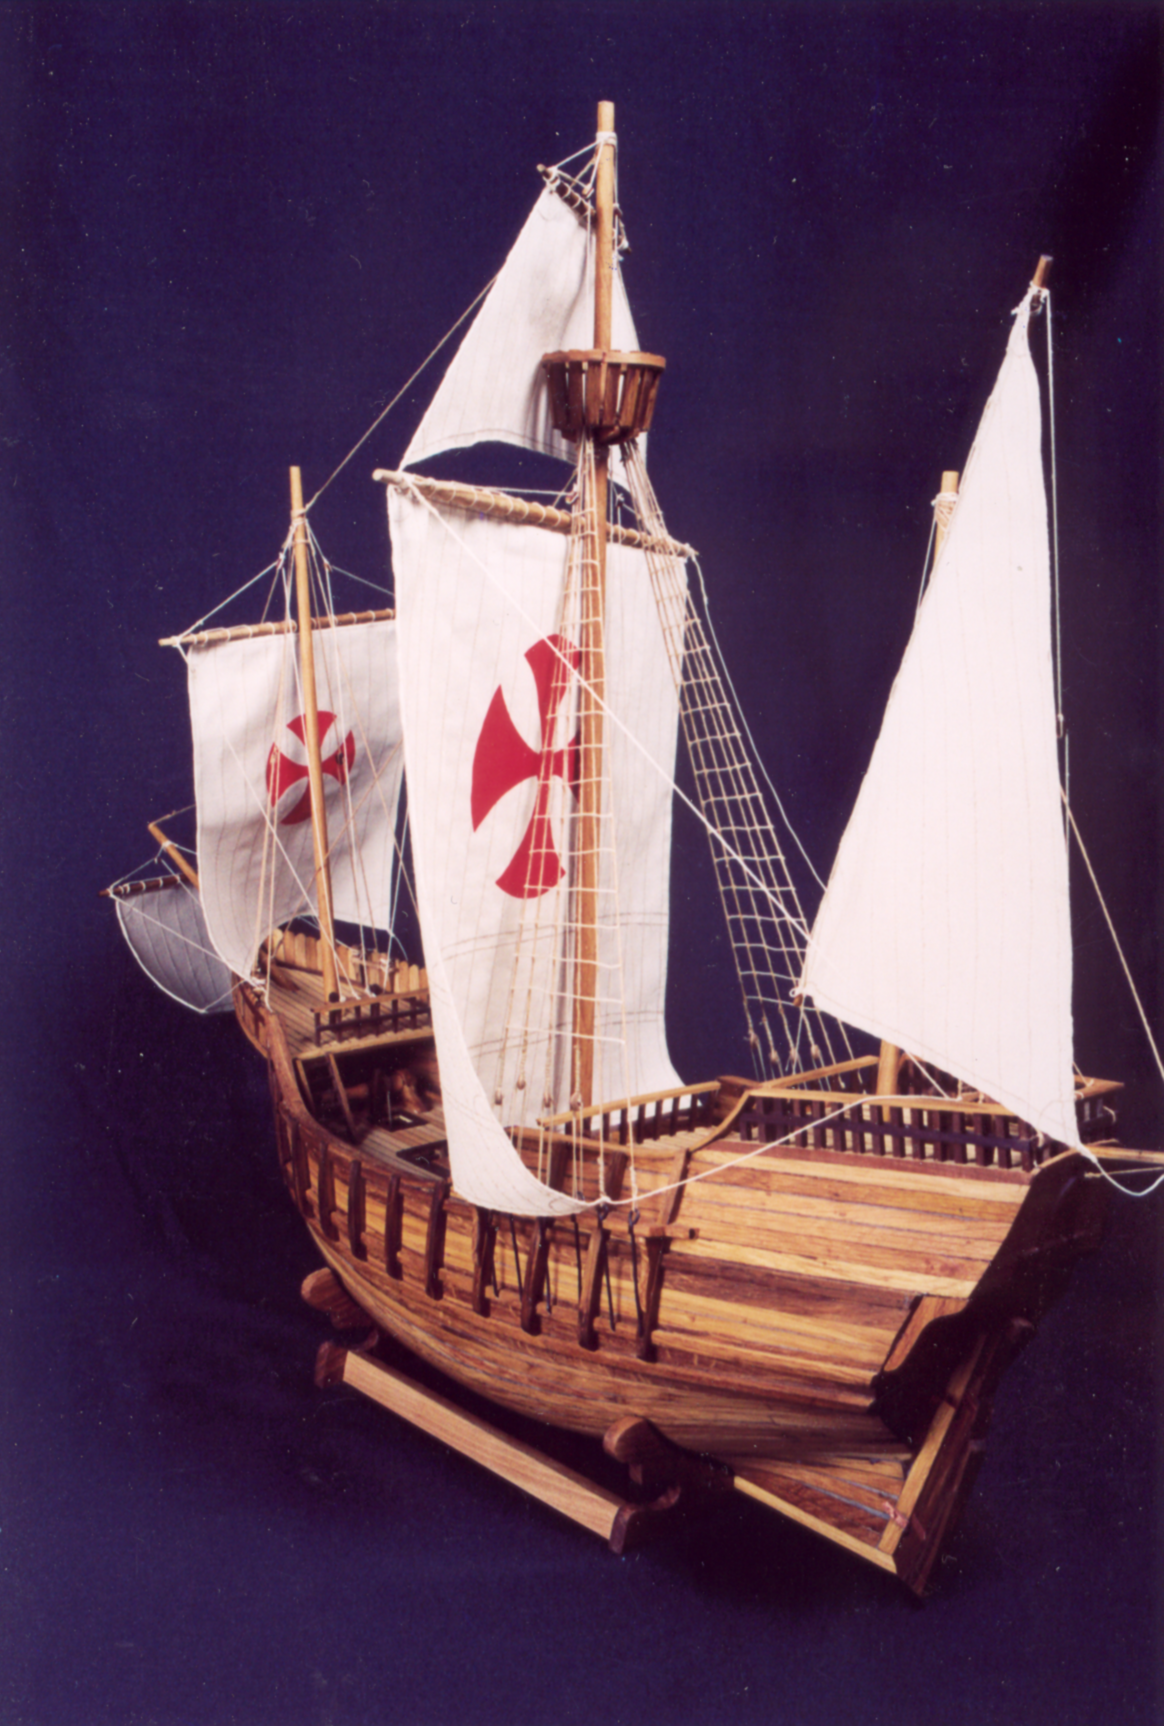
\includegraphics[width=\textwidth]{../results/task3_gauss08_SantaMaria.png}
        \caption{Gauss $\sigma=0.8$}
    \end{subfigure}
    \begin{subfigure}[b]{0.32\textwidth}
        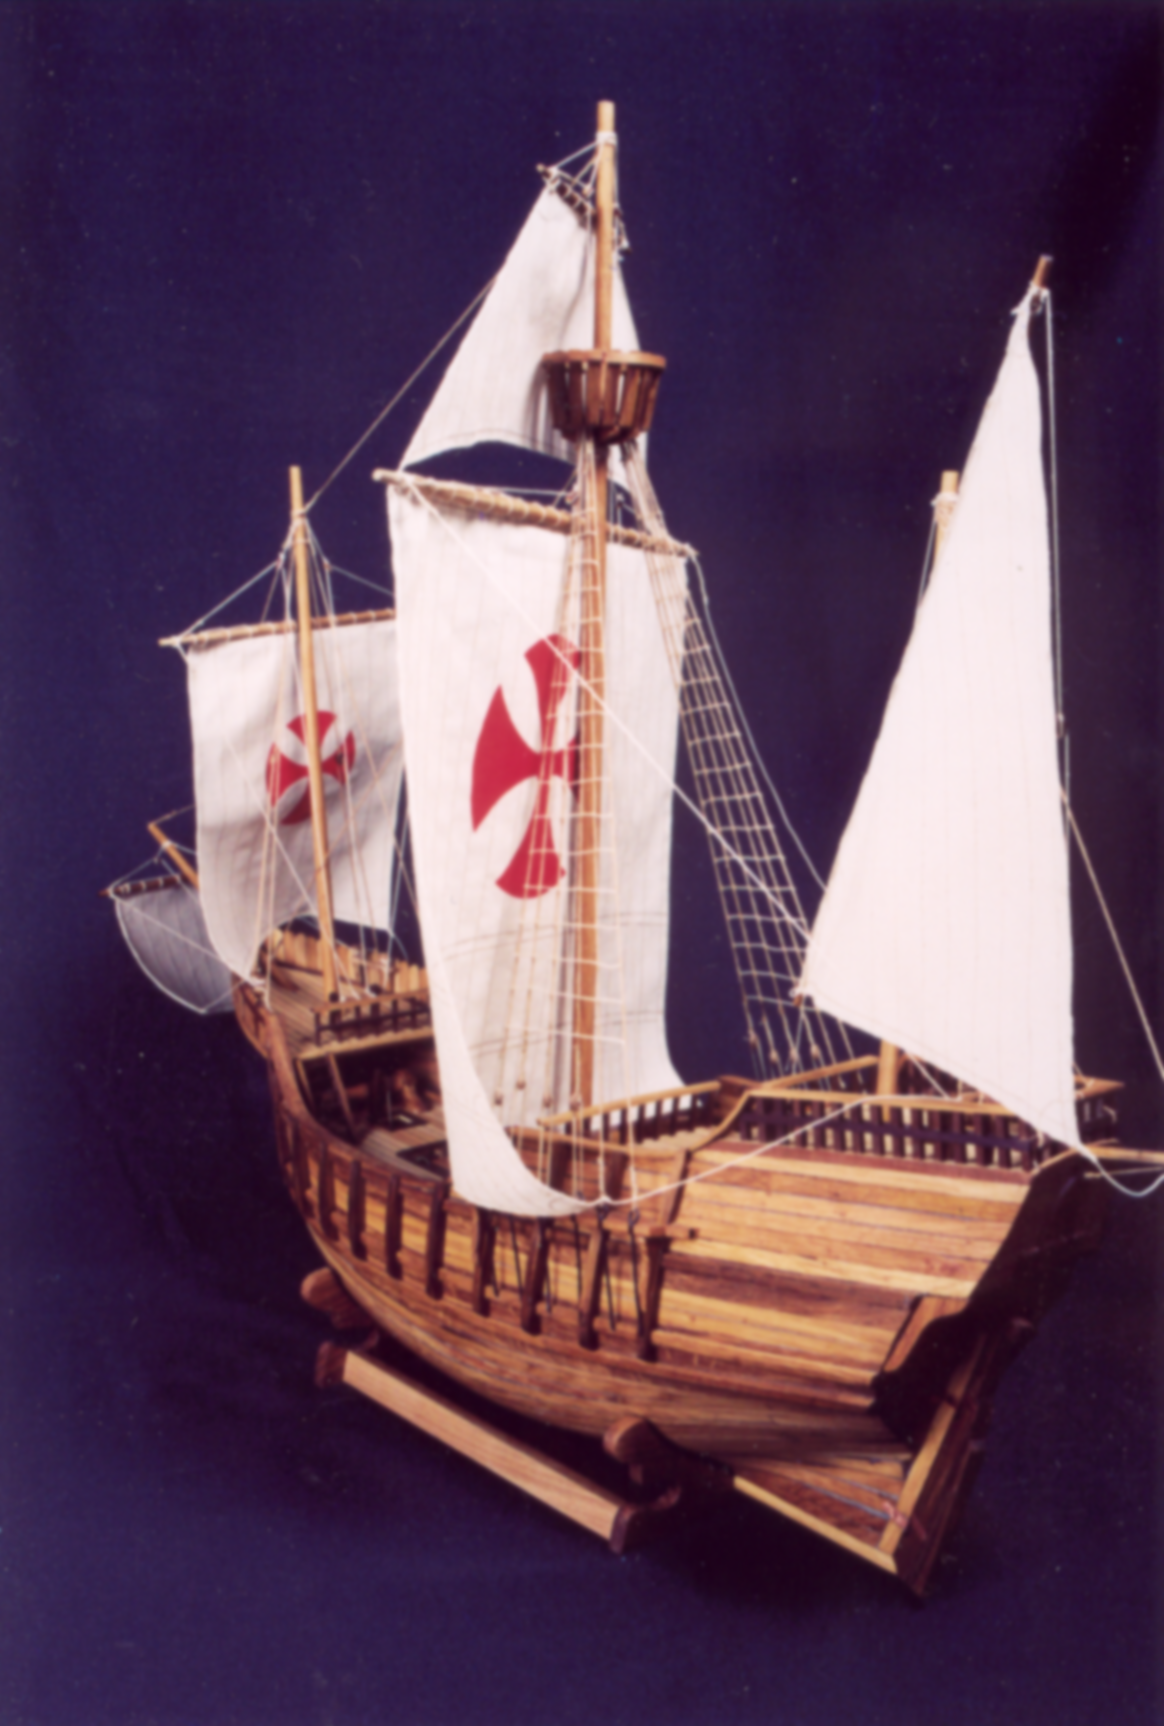
\includegraphics[width=\textwidth]{../results/task3_gauss18_SantaMaria.png}
        \caption{Gauss $\sigma=1.8$}
    \end{subfigure}
    \begin{subfigure}[b]{0.32\textwidth}
        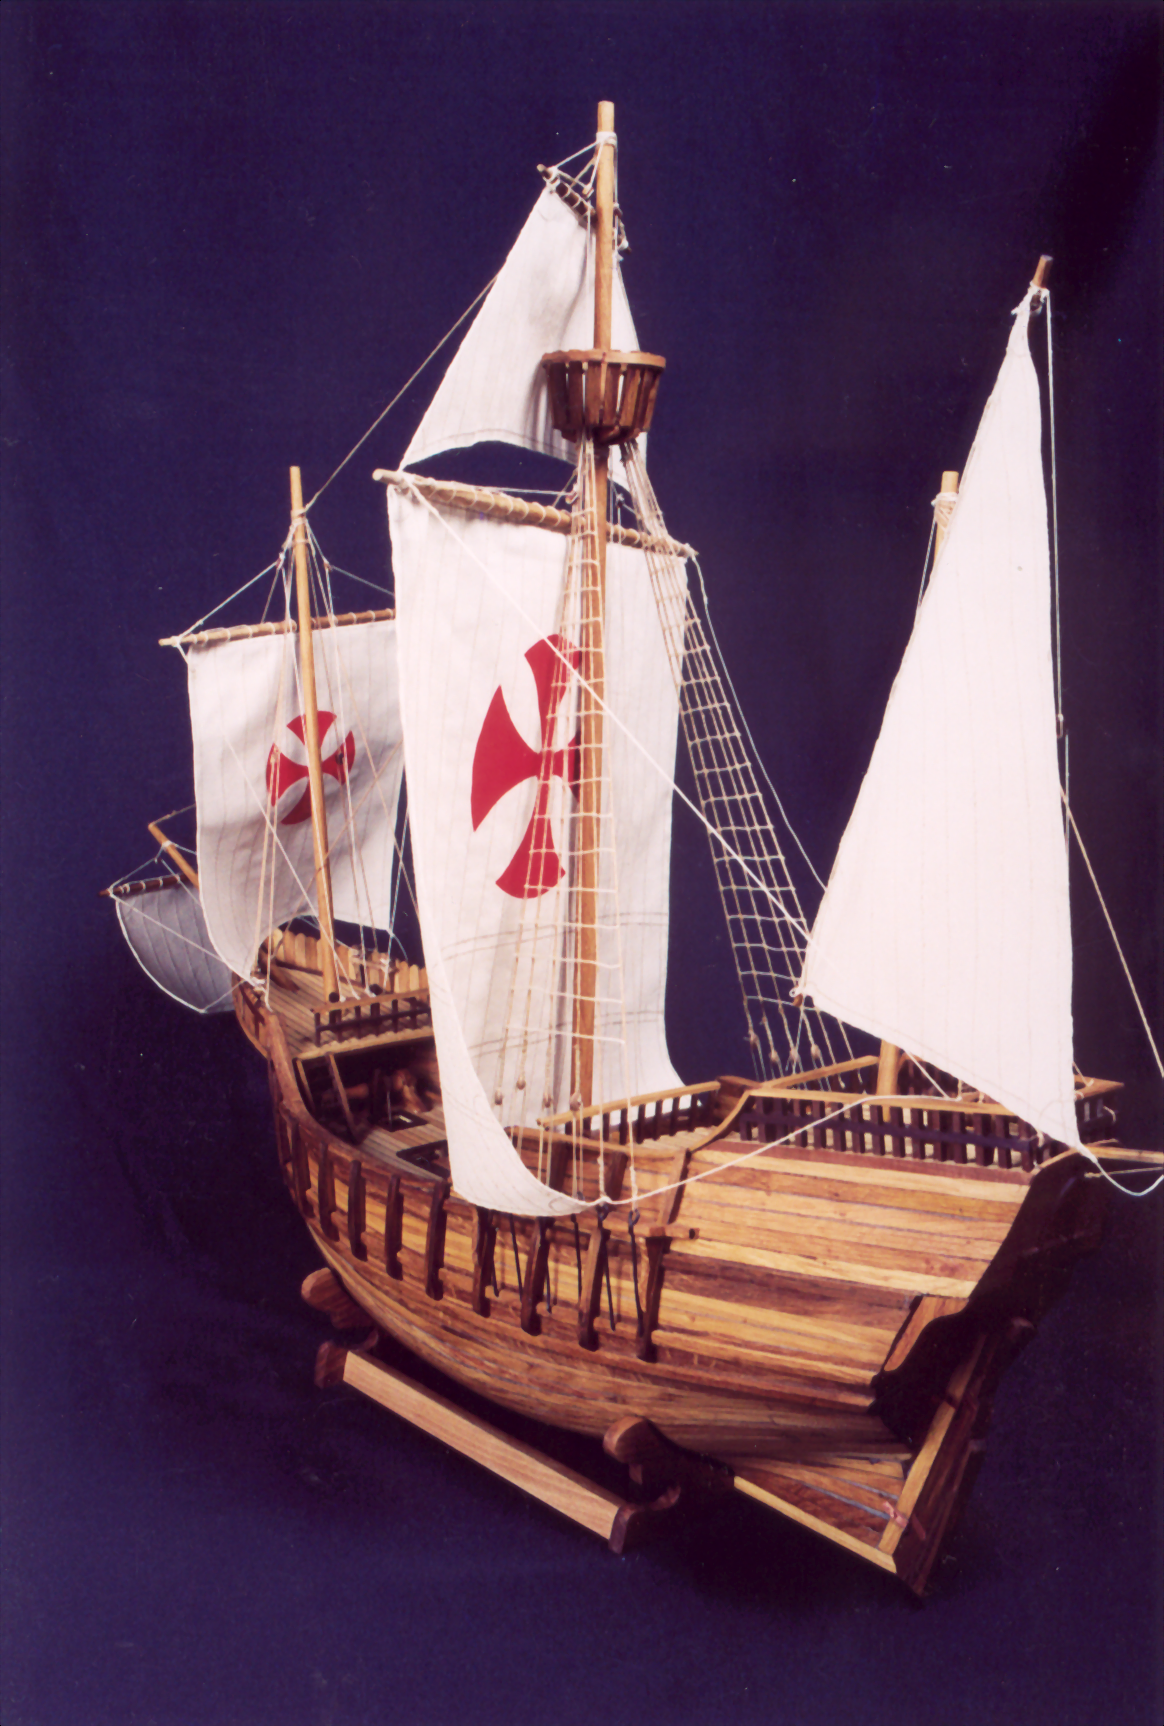
\includegraphics[width=\textwidth]{../results/task3_median3_SantaMaria.png}
        \caption{Median 3$\times$3}
    \end{subfigure}
    \caption{SantaMaria.tif – индивидуални резултати от филтриране}
\end{figure}

\noindent Таблица с качествена оценка:

\begin{table}[H]
\centering
\caption{Качествена оценка на изглаждащите филтри}
\begin{tabular}{lllll}
\toprule
\textbf{Филтър} & \textbf{Параметри} & \textbf{Шум} & \textbf{Ръбове} & \textbf{Детайли} \\
\midrule
Mean      & 5$\times$5   & Умерено намален & Леко замъглени  & Леко изгубени \\
Mean      & 11$\times$11 & Значително намален & Силно замъглени & Значително изгубени \\
Gaussian  & $\sigma=0.8$ & Леко намален   & Добре запазени  & Добре запазени \\
Gaussian  & $\sigma=1.8$ & Умерено намален & Умерено замъглени & Умерено изгубени \\
Median    & 3$\times$3   & Добре намален   & Добре запазени  & Добре запазени \\
Median    & 7$\times$7   & Значително намален & Умерено замъглени & Умерено изгубени \\
\bottomrule
\end{tabular}
\end{table}

\subsubsection{Анализ}

\textbf{Влияние на различните филтри:}
\begin{itemize}
    \item \textbf{Шум:} Всички три вида филтри намаляват шума, но по различен начин. Медианният филтър е особено ефективен при импулсен (salt-and-pepper) шум. Осредняващият и Гаусовият намаляват гаусов шум равномерно.
    \item \textbf{Ръбове:} Осредняващият филтър с голяма маска (11$\times$11) силно замъглява ръбовете. Гаусовият с малко $\sigma$ и медианният 3$\times$3 запазват ръбовете по-добре.
    \item \textbf{Фини текстури:} Медианният филтър запазва по-добре фините текстури в сравнение с осредняващия при еднакво ниво на изглаждане.
\end{itemize}

\textbf{Осредняващ срещу Гаусов:} При сходно ниво на изглаждане Гаусовият филтър запазва по-добре структурата на ръбовете, тъй като намалява теглото на периферните пиксели в маската. Осредняващият третира всички пиксели в маската еднакво, което води до по-изразено замъгляване.

\textbf{Предимство на медианния филтър:} Медианният филтър е нелинеен и не въвежда нови стойности в изображението. Това го прави особено подходящ при наличие на импулсен шум, тъй като замества екстремните стойности с медианата на съседите, без да замъглява рязко ръбовете.

\textbf{Пример за прекомерно изглаждане:} Mean 11$\times$11 при SantaMaria.tif – детайлите на корабните мачти и текстурата на водата почти напълно изчезват.

\subsection{Задание 4 – Засилване на рязкостта (Unsharp Masking)}

\subsubsection{Код}

\begin{lstlisting}[language=Matlab, caption={task4\_unsharp.m}]
pkg load image;
clear; close all;

img_dir = '../images/';
out_dir = '../results/';
alphas = [0.3, 0.7, 1.2];

function process_unsharp(img_input, tag, alphas, out_dir)
    img_base = im2uint8(img_input);
    sigma_blur = 1.5;
    h_blur = fspecial('gaussian', [9 9], sigma_blur);
    if size(img_base, 3) == 3
        img_blurred = cat(3, imfilter(img_base(:,:,1), h_blur, 'replicate'), ...
                             imfilter(img_base(:,:,2), h_blur, 'replicate'), ...
                             imfilter(img_base(:,:,3), h_blur, 'replicate'));
    else
        img_blurred = imfilter(img_base, h_blur, 'replicate');
    end
    img_sharp = cell(1, length(alphas));
    for i = 1:length(alphas)
        alpha = alphas(i);
        mask = double(img_base) - double(img_blurred);
        sharpened = double(img_base) + alpha * mask;
        img_sharp{i} = uint8(min(max(sharpened, 0), 255));
    end
    imwrite(img_base,     [out_dir 'task4_original_'    tag '.png']);
    imwrite(img_sharp{1}, [out_dir 'task4_unsharp_a03_' tag '.png']);
    imwrite(img_sharp{2}, [out_dir 'task4_unsharp_a07_' tag '.png']);
    imwrite(img_sharp{3}, [out_dir 'task4_unsharp_a12_' tag '.png']);
    fig = figure('visible', 'off', 'Position', [0 0 1200 400]);
    all_imgs   = {img_base, img_sharp{1}, img_sharp{2}, img_sharp{3}};
    all_titles = {'Original', 'alpha=0.3', 'alpha=0.7', 'alpha=1.2'};
    for i = 1:4
        subplot(1, 4, i); imshow(all_imgs{i}); title(all_titles{i});
    end
    saveas(fig, [out_dir 'task4_comparison_' tag '.png']);
    close(fig);
end

% Image 1: ImgTestSharp.tif
img1 = imread([img_dir 'ImgTestSharp.tif']);
if size(img1, 3) == 3; img1 = rgb2gray(img1); end
process_unsharp(img1, 'ImgTestSharp', alphas, out_dir);

% Image 2: America.tif pre-smoothed with Gaussian sigma=1.8 (Task 3)
img2 = imread([img_dir 'America.tif']);
hg18 = fspecial('gaussian', [21 21], 1.8);
img2_smoothed = cat(3, imfilter(img2(:,:,1), hg18, 'replicate'), ...
                       imfilter(img2(:,:,2), hg18, 'replicate'), ...
                       imfilter(img2(:,:,3), hg18, 'replicate'));
process_unsharp(img2_smoothed, 'America', alphas, out_dir);
\end{lstlisting}

\subsubsection{Резултати}

Методът Unsharp Masking е приложен върху две изображения при $\alpha = 0.3$, $\alpha = 0.7$ и $\alpha = 1.2$. Формулата е: $I_{\text{sharp}} = I + \alpha \cdot (I - I_{\text{blur}})$.

\noindent\textbf{Изображение 1: ImgTestSharp.tif}

\begin{figure}[H]
    \centering
    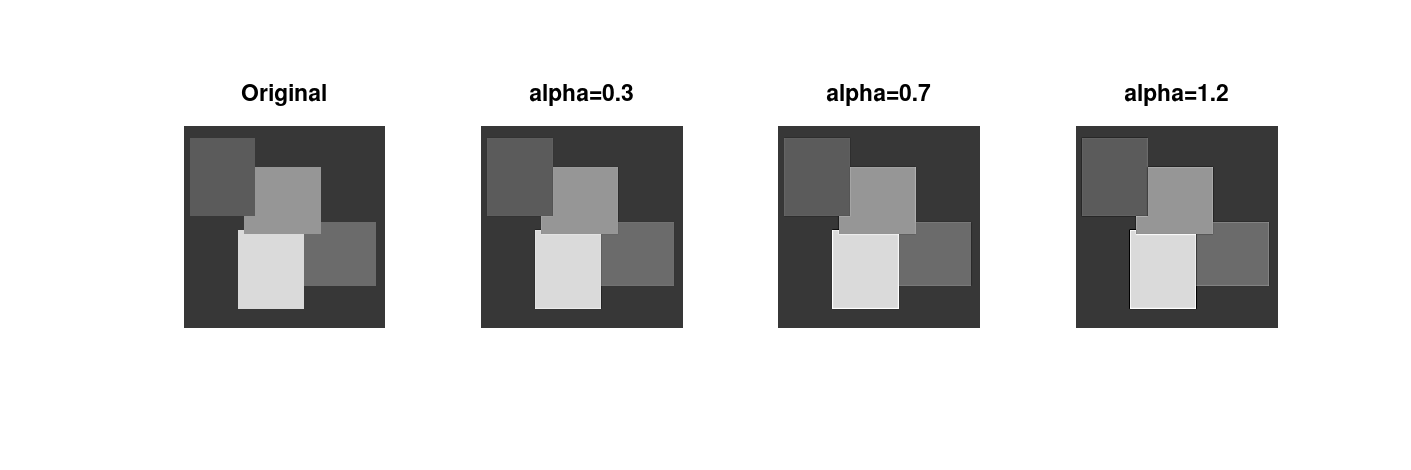
\includegraphics[width=\textwidth]{../results/task4_comparison_ImgTestSharp.png}
    \caption{ImgTestSharp.tif – сравнение: оригинал, $\alpha=0.3$, $\alpha=0.7$, $\alpha=1.2$}
\end{figure}

\begin{figure}[H]
    \centering
    \begin{subfigure}[b]{0.22\textwidth}
        
\includegraphics[width=\textwidth]{../results/task4_original_ImgTestSharp.png}
        \caption{Оригинал}
    \end{subfigure}
    \begin{subfigure}[b]{0.22\textwidth}
        
\includegraphics[width=\textwidth]{../results/task4_unsharp_a03_ImgTestSharp.png}
        \caption{$\alpha=0.3$}
    \end{subfigure}
    \begin{subfigure}[b]{0.22\textwidth}
        
\includegraphics[width=\textwidth]{../results/task4_unsharp_a07_ImgTestSharp.png}
        \caption{$\alpha=0.7$}
    \end{subfigure}
    \begin{subfigure}[b]{0.22\textwidth}
        
\includegraphics[width=\textwidth]{../results/task4_unsharp_a12_ImgTestSharp.png}
        \caption{$\alpha=1.2$}
    \end{subfigure}
    \caption{ImgTestSharp.tif – Unsharp Masking при различни стойности на $\alpha$}
\end{figure}

\noindent\textbf{Изображение 2: America.tif (предварително изгладено с Гаусов филтър $\sigma=1.8$ от Задание 3)}

\begin{figure}[H]
    \centering
    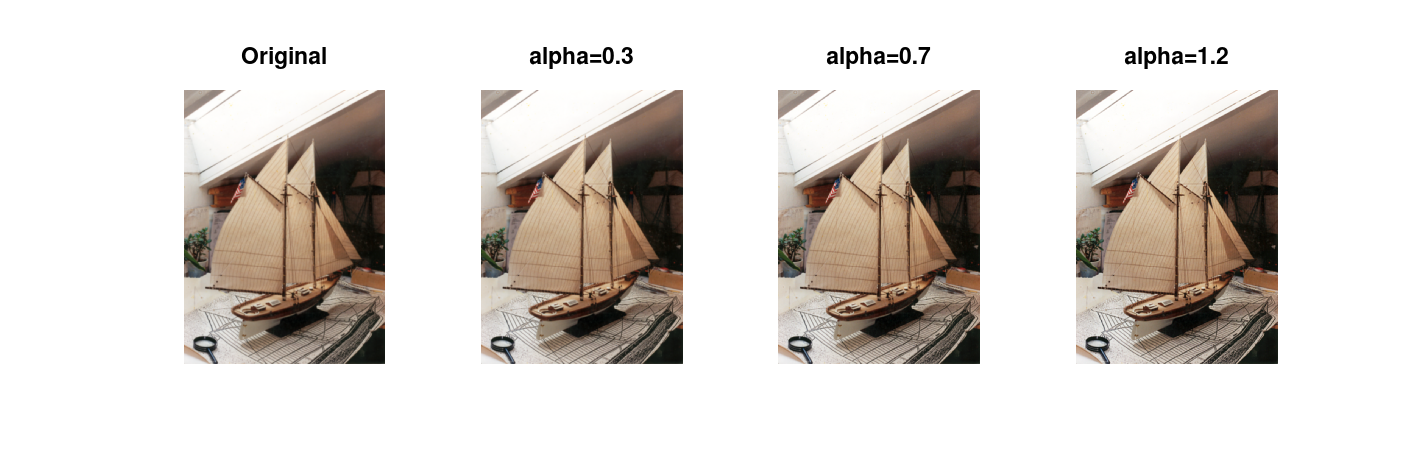
\includegraphics[width=\textwidth]{../results/task4_comparison_America.png}
    \caption{America.tif (изгладено) – сравнение: оригинал, $\alpha=0.3$, $\alpha=0.7$, $\alpha=1.2$}
\end{figure}

\begin{figure}[H]
    \centering
    \begin{subfigure}[b]{0.22\textwidth}
        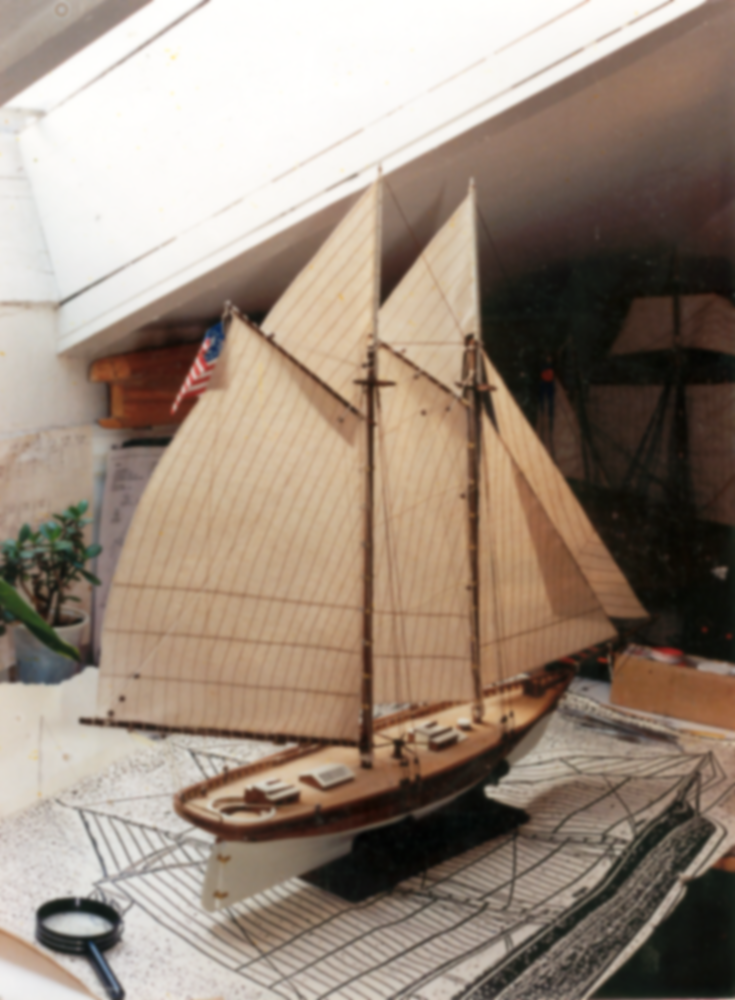
\includegraphics[width=\textwidth]{../results/task4_original_America.png}
        \caption{Изгладено}
    \end{subfigure}
    \begin{subfigure}[b]{0.22\textwidth}
        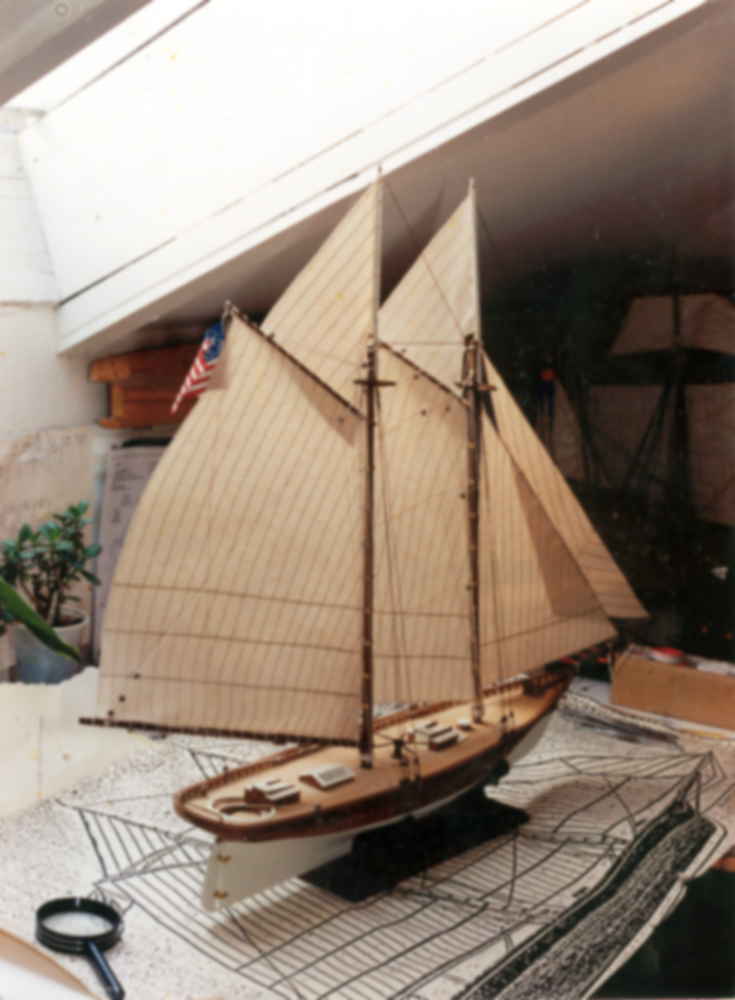
\includegraphics[width=\textwidth]{../results/task4_unsharp_a03_America.png}
        \caption{$\alpha=0.3$}
    \end{subfigure}
    \begin{subfigure}[b]{0.22\textwidth}
        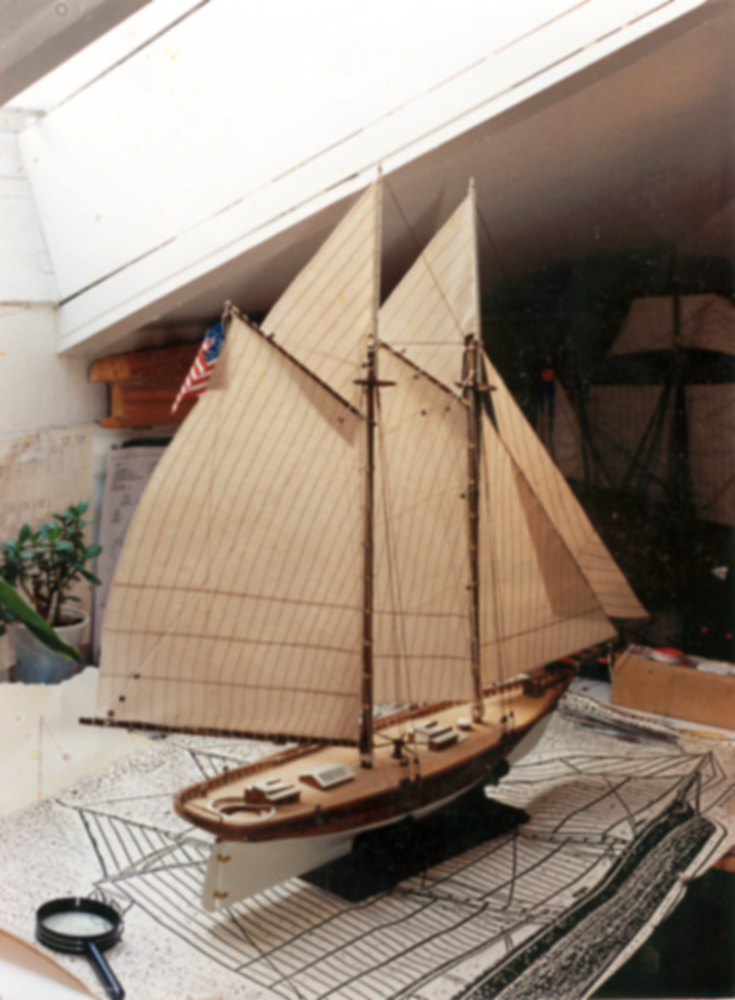
\includegraphics[width=\textwidth]{../results/task4_unsharp_a07_America.png}
        \caption{$\alpha=0.7$}
    \end{subfigure}
    \begin{subfigure}[b]{0.22\textwidth}
        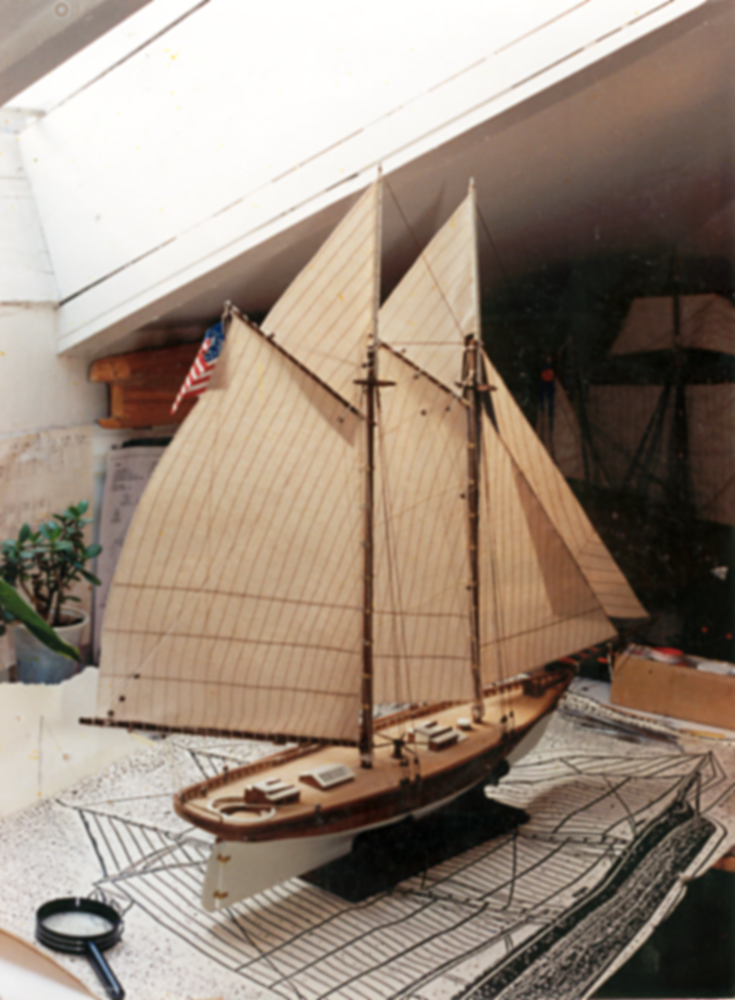
\includegraphics[width=\textwidth]{../results/task4_unsharp_a12_America.png}
        \caption{$\alpha=1.2$}
    \end{subfigure}
    \caption{America.tif (изгладено, $\sigma=1.8$) – Unsharp Masking при различни стойности на $\alpha$}
\end{figure}

\subsubsection{Анализ}

\textbf{Ефект на увеличаване на $\alpha$:}
\begin{itemize}
    \item \textbf{Ръбове:} С нарастване на $\alpha$ ръбовете стават все по-изразени и с по-висок контраст. При $\alpha=1.2$ ръбовете са рязко подчертани.
    \item \textbf{Детайли:} Малките детайли и текстури стават по-видими с нарастване на $\alpha$.
    \item \textbf{Шум:} Всеки шум в оригиналното изображение се усилва заедно с ръбовете, тъй като маската $I - I_{\text{blur}}$ съдържа и шумови компоненти.
\end{itemize}

\textbf{Артефакти:}
\begin{itemize}
    \item \textbf{Ореоли (halos):} При $\alpha=1.2$ се наблюдават ореоли около ръбовете – характерни светли/тъмни ивици по двете страни на прехода.
    \item \textbf{Неестествен контраст:} При висок $\alpha$ локалният контраст може да стане неестествено висок.
    \item \textbf{Усилен шум:} При $\alpha=1.2$ шумовите пиксели са видимо усилени в сравнение с оригинала.
\end{itemize}

\textbf{Най-подходяща стойност:} $\alpha = 0.7$ предлага добър баланс – ръбовете са ясно подчертани, детайлите са видими, без прекомерни ореоли. При ImgTestSharp.tif това изявява структурите на ръбовете. При изгладеното America.tif $\alpha = 0.7$ частично възстановява детайлите на корпуса и мачтите на кораба, загубени при изглаждането.

\textbf{Сравнение между двете изображения:} При ImgTestSharp.tif (минимален шум) ефектът от Unsharp Masking е чист – ръбовете се подчертават без нежелани артефакти. При изгладеното America.tif (с вече намален шум от Гаусовия филтър) Unsharp Masking при $\alpha = 0.7$ успешно компенсира изглаждането, а при $\alpha = 1.2$ се появяват видими ореоли около ребрата на кораба.

\textbf{Прекомерно засилване:} $\alpha = 1.2$ е пример за прекомерно засилване – ореолите около ръбовете са видими с невъоръжено око и намаляват естествения изглед. При America.tif артефактите са особено забележими около контрастните ръбове на кораба и хоризонта.

\section{Общи изводи}

\textbf{Хистограма и визуално възприятие:} Хистограмата е директен показател за яркостното разпределение. Концентрирана хистограма в тесен диапазон означава нисък контраст; равномерно разпределена хистограма – висок контраст. Визуалното възприятие корелира добре с тези статистически мерки.

\textbf{Линейни и нелинейни трансформации:} imadjust (линейна трансформация) разтяга хистограмата равномерно. $\gamma$-корекцията (нелинейна) позволява селективно засилване на тъмните ($\gamma < 1$) или светлите ($\gamma > 1$) области. Нелинейните трансформации предлагат по-голям контрол върху конкретни тонални области.

\textbf{Сравнение на изглаждащи филтри:} Медианният филтър е най-добър при импулсен шум. Гаусовият запазва по-добре ръбовете в сравнение с осредняващия при еднакво изглаждане. Осредняващият е прост и ефективен за гаусов шум, но силно замъглява ръбовете.

\textbf{Компромис между шум, рязкост и детайли:} Всяко изглаждане неизбежно намалява рязкостта. Unsharp Masking позволява да се върне рязкостта след изглаждане, но усилва и шума. Изборът на метод и параметри е компромис между тези три характеристики.

\textbf{Влияние на параметрите:}
\begin{itemize}
    \item $\gamma$: контролира кои тонални области се засилват.
    \item $\sigma$ (Гаус): контролира степента на изглаждане и обхвата на влияние.
    \item Размер на маска: по-голяма маска $\Rightarrow$ по-силно изглаждане, но повече замъгляване.
    \item $\alpha$ (Unsharp Masking): контролира степента на засилване на ръбовете.
\end{itemize}

\textbf{Кога кой метод е най-подходящ:}
\begin{itemize}
    \item Нисък контраст – imadjust или $\gamma$-корекция.
    \item Импулсен шум – медианен филтър.
    \item Гаусов шум – Гаусов или осредняващ филтър.
    \item Засилване на детайли – Unsharp Masking с подходящо $\alpha$.
\end{itemize}
